
% Default to the notebook output style

    


% Inherit from the specified cell style.




    
\documentclass[11pt]{article}

    
    
    \usepackage[T1]{fontenc}
    % Nicer default font (+ math font) than Computer Modern for most use cases
    \usepackage{mathpazo}

    % Basic figure setup, for now with no caption control since it's done
    % automatically by Pandoc (which extracts ![](path) syntax from Markdown).
    \usepackage{graphicx}
    % We will generate all images so they have a width \maxwidth. This means
    % that they will get their normal width if they fit onto the page, but
    % are scaled down if they would overflow the margins.
    \makeatletter
    \def\maxwidth{\ifdim\Gin@nat@width>\linewidth\linewidth
    \else\Gin@nat@width\fi}
    \makeatother
    \let\Oldincludegraphics\includegraphics
    % Set max figure width to be 80% of text width, for now hardcoded.
    \renewcommand{\includegraphics}[1]{\Oldincludegraphics[width=.8\maxwidth]{#1}}
    % Ensure that by default, figures have no caption (until we provide a
    % proper Figure object with a Caption API and a way to capture that
    % in the conversion process - todo).
    \usepackage{caption}
    \DeclareCaptionLabelFormat{nolabel}{}
    \captionsetup{labelformat=nolabel}

    \usepackage{adjustbox} % Used to constrain images to a maximum size 
    \usepackage{xcolor} % Allow colors to be defined
    \usepackage{enumerate} % Needed for markdown enumerations to work
    \usepackage{geometry} % Used to adjust the document margins
    \usepackage{amsmath} % Equations
    \usepackage{amssymb} % Equations
    \usepackage{textcomp} % defines textquotesingle
    % Hack from http://tex.stackexchange.com/a/47451/13684:
    \AtBeginDocument{%
        \def\PYZsq{\textquotesingle}% Upright quotes in Pygmentized code
    }
    \usepackage{upquote} % Upright quotes for verbatim code
    \usepackage{eurosym} % defines \euro
    \usepackage[mathletters]{ucs} % Extended unicode (utf-8) support
    \usepackage[utf8x]{inputenc} % Allow utf-8 characters in the tex document
    \usepackage{fancyvrb} % verbatim replacement that allows latex
    \usepackage{grffile} % extends the file name processing of package graphics 
                         % to support a larger range 
    % The hyperref package gives us a pdf with properly built
    % internal navigation ('pdf bookmarks' for the table of contents,
    % internal cross-reference links, web links for URLs, etc.)
    \usepackage{hyperref}
    \usepackage{longtable} % longtable support required by pandoc >1.10
    \usepackage{booktabs}  % table support for pandoc > 1.12.2
    \usepackage[inline]{enumitem} % IRkernel/repr support (it uses the enumerate* environment)
    \usepackage[normalem]{ulem} % ulem is needed to support strikethroughs (\sout)
                                % normalem makes italics be italics, not underlines
    

    
    
    % Colors for the hyperref package
    \definecolor{urlcolor}{rgb}{0,.145,.698}
    \definecolor{linkcolor}{rgb}{.71,0.21,0.01}
    \definecolor{citecolor}{rgb}{.12,.54,.11}

    % ANSI colors
    \definecolor{ansi-black}{HTML}{3E424D}
    \definecolor{ansi-black-intense}{HTML}{282C36}
    \definecolor{ansi-red}{HTML}{E75C58}
    \definecolor{ansi-red-intense}{HTML}{B22B31}
    \definecolor{ansi-green}{HTML}{00A250}
    \definecolor{ansi-green-intense}{HTML}{007427}
    \definecolor{ansi-yellow}{HTML}{DDB62B}
    \definecolor{ansi-yellow-intense}{HTML}{B27D12}
    \definecolor{ansi-blue}{HTML}{208FFB}
    \definecolor{ansi-blue-intense}{HTML}{0065CA}
    \definecolor{ansi-magenta}{HTML}{D160C4}
    \definecolor{ansi-magenta-intense}{HTML}{A03196}
    \definecolor{ansi-cyan}{HTML}{60C6C8}
    \definecolor{ansi-cyan-intense}{HTML}{258F8F}
    \definecolor{ansi-white}{HTML}{C5C1B4}
    \definecolor{ansi-white-intense}{HTML}{A1A6B2}

    % commands and environments needed by pandoc snippets
    % extracted from the output of `pandoc -s`
    \providecommand{\tightlist}{%
      \setlength{\itemsep}{0pt}\setlength{\parskip}{0pt}}
    \DefineVerbatimEnvironment{Highlighting}{Verbatim}{commandchars=\\\{\}}
    % Add ',fontsize=\small' for more characters per line
    \newenvironment{Shaded}{}{}
    \newcommand{\KeywordTok}[1]{\textcolor[rgb]{0.00,0.44,0.13}{\textbf{{#1}}}}
    \newcommand{\DataTypeTok}[1]{\textcolor[rgb]{0.56,0.13,0.00}{{#1}}}
    \newcommand{\DecValTok}[1]{\textcolor[rgb]{0.25,0.63,0.44}{{#1}}}
    \newcommand{\BaseNTok}[1]{\textcolor[rgb]{0.25,0.63,0.44}{{#1}}}
    \newcommand{\FloatTok}[1]{\textcolor[rgb]{0.25,0.63,0.44}{{#1}}}
    \newcommand{\CharTok}[1]{\textcolor[rgb]{0.25,0.44,0.63}{{#1}}}
    \newcommand{\StringTok}[1]{\textcolor[rgb]{0.25,0.44,0.63}{{#1}}}
    \newcommand{\CommentTok}[1]{\textcolor[rgb]{0.38,0.63,0.69}{\textit{{#1}}}}
    \newcommand{\OtherTok}[1]{\textcolor[rgb]{0.00,0.44,0.13}{{#1}}}
    \newcommand{\AlertTok}[1]{\textcolor[rgb]{1.00,0.00,0.00}{\textbf{{#1}}}}
    \newcommand{\FunctionTok}[1]{\textcolor[rgb]{0.02,0.16,0.49}{{#1}}}
    \newcommand{\RegionMarkerTok}[1]{{#1}}
    \newcommand{\ErrorTok}[1]{\textcolor[rgb]{1.00,0.00,0.00}{\textbf{{#1}}}}
    \newcommand{\NormalTok}[1]{{#1}}
    
    % Additional commands for more recent versions of Pandoc
    \newcommand{\ConstantTok}[1]{\textcolor[rgb]{0.53,0.00,0.00}{{#1}}}
    \newcommand{\SpecialCharTok}[1]{\textcolor[rgb]{0.25,0.44,0.63}{{#1}}}
    \newcommand{\VerbatimStringTok}[1]{\textcolor[rgb]{0.25,0.44,0.63}{{#1}}}
    \newcommand{\SpecialStringTok}[1]{\textcolor[rgb]{0.73,0.40,0.53}{{#1}}}
    \newcommand{\ImportTok}[1]{{#1}}
    \newcommand{\DocumentationTok}[1]{\textcolor[rgb]{0.73,0.13,0.13}{\textit{{#1}}}}
    \newcommand{\AnnotationTok}[1]{\textcolor[rgb]{0.38,0.63,0.69}{\textbf{\textit{{#1}}}}}
    \newcommand{\CommentVarTok}[1]{\textcolor[rgb]{0.38,0.63,0.69}{\textbf{\textit{{#1}}}}}
    \newcommand{\VariableTok}[1]{\textcolor[rgb]{0.10,0.09,0.49}{{#1}}}
    \newcommand{\ControlFlowTok}[1]{\textcolor[rgb]{0.00,0.44,0.13}{\textbf{{#1}}}}
    \newcommand{\OperatorTok}[1]{\textcolor[rgb]{0.40,0.40,0.40}{{#1}}}
    \newcommand{\BuiltInTok}[1]{{#1}}
    \newcommand{\ExtensionTok}[1]{{#1}}
    \newcommand{\PreprocessorTok}[1]{\textcolor[rgb]{0.74,0.48,0.00}{{#1}}}
    \newcommand{\AttributeTok}[1]{\textcolor[rgb]{0.49,0.56,0.16}{{#1}}}
    \newcommand{\InformationTok}[1]{\textcolor[rgb]{0.38,0.63,0.69}{\textbf{\textit{{#1}}}}}
    \newcommand{\WarningTok}[1]{\textcolor[rgb]{0.38,0.63,0.69}{\textbf{\textit{{#1}}}}}
    
    
    % Define a nice break command that doesn't care if a line doesn't already
    % exist.
    \def\br{\hspace*{\fill} \\* }
    % Math Jax compatability definitions
    \def\gt{>}
    \def\lt{<}
    % Document parameters
    \title{Chapter 3}
    
    
    

    % Pygments definitions
    
\makeatletter
\def\PY@reset{\let\PY@it=\relax \let\PY@bf=\relax%
    \let\PY@ul=\relax \let\PY@tc=\relax%
    \let\PY@bc=\relax \let\PY@ff=\relax}
\def\PY@tok#1{\csname PY@tok@#1\endcsname}
\def\PY@toks#1+{\ifx\relax#1\empty\else%
    \PY@tok{#1}\expandafter\PY@toks\fi}
\def\PY@do#1{\PY@bc{\PY@tc{\PY@ul{%
    \PY@it{\PY@bf{\PY@ff{#1}}}}}}}
\def\PY#1#2{\PY@reset\PY@toks#1+\relax+\PY@do{#2}}

\expandafter\def\csname PY@tok@w\endcsname{\def\PY@tc##1{\textcolor[rgb]{0.73,0.73,0.73}{##1}}}
\expandafter\def\csname PY@tok@c\endcsname{\let\PY@it=\textit\def\PY@tc##1{\textcolor[rgb]{0.25,0.50,0.50}{##1}}}
\expandafter\def\csname PY@tok@cp\endcsname{\def\PY@tc##1{\textcolor[rgb]{0.74,0.48,0.00}{##1}}}
\expandafter\def\csname PY@tok@k\endcsname{\let\PY@bf=\textbf\def\PY@tc##1{\textcolor[rgb]{0.00,0.50,0.00}{##1}}}
\expandafter\def\csname PY@tok@kp\endcsname{\def\PY@tc##1{\textcolor[rgb]{0.00,0.50,0.00}{##1}}}
\expandafter\def\csname PY@tok@kt\endcsname{\def\PY@tc##1{\textcolor[rgb]{0.69,0.00,0.25}{##1}}}
\expandafter\def\csname PY@tok@o\endcsname{\def\PY@tc##1{\textcolor[rgb]{0.40,0.40,0.40}{##1}}}
\expandafter\def\csname PY@tok@ow\endcsname{\let\PY@bf=\textbf\def\PY@tc##1{\textcolor[rgb]{0.67,0.13,1.00}{##1}}}
\expandafter\def\csname PY@tok@nb\endcsname{\def\PY@tc##1{\textcolor[rgb]{0.00,0.50,0.00}{##1}}}
\expandafter\def\csname PY@tok@nf\endcsname{\def\PY@tc##1{\textcolor[rgb]{0.00,0.00,1.00}{##1}}}
\expandafter\def\csname PY@tok@nc\endcsname{\let\PY@bf=\textbf\def\PY@tc##1{\textcolor[rgb]{0.00,0.00,1.00}{##1}}}
\expandafter\def\csname PY@tok@nn\endcsname{\let\PY@bf=\textbf\def\PY@tc##1{\textcolor[rgb]{0.00,0.00,1.00}{##1}}}
\expandafter\def\csname PY@tok@ne\endcsname{\let\PY@bf=\textbf\def\PY@tc##1{\textcolor[rgb]{0.82,0.25,0.23}{##1}}}
\expandafter\def\csname PY@tok@nv\endcsname{\def\PY@tc##1{\textcolor[rgb]{0.10,0.09,0.49}{##1}}}
\expandafter\def\csname PY@tok@no\endcsname{\def\PY@tc##1{\textcolor[rgb]{0.53,0.00,0.00}{##1}}}
\expandafter\def\csname PY@tok@nl\endcsname{\def\PY@tc##1{\textcolor[rgb]{0.63,0.63,0.00}{##1}}}
\expandafter\def\csname PY@tok@ni\endcsname{\let\PY@bf=\textbf\def\PY@tc##1{\textcolor[rgb]{0.60,0.60,0.60}{##1}}}
\expandafter\def\csname PY@tok@na\endcsname{\def\PY@tc##1{\textcolor[rgb]{0.49,0.56,0.16}{##1}}}
\expandafter\def\csname PY@tok@nt\endcsname{\let\PY@bf=\textbf\def\PY@tc##1{\textcolor[rgb]{0.00,0.50,0.00}{##1}}}
\expandafter\def\csname PY@tok@nd\endcsname{\def\PY@tc##1{\textcolor[rgb]{0.67,0.13,1.00}{##1}}}
\expandafter\def\csname PY@tok@s\endcsname{\def\PY@tc##1{\textcolor[rgb]{0.73,0.13,0.13}{##1}}}
\expandafter\def\csname PY@tok@sd\endcsname{\let\PY@it=\textit\def\PY@tc##1{\textcolor[rgb]{0.73,0.13,0.13}{##1}}}
\expandafter\def\csname PY@tok@si\endcsname{\let\PY@bf=\textbf\def\PY@tc##1{\textcolor[rgb]{0.73,0.40,0.53}{##1}}}
\expandafter\def\csname PY@tok@se\endcsname{\let\PY@bf=\textbf\def\PY@tc##1{\textcolor[rgb]{0.73,0.40,0.13}{##1}}}
\expandafter\def\csname PY@tok@sr\endcsname{\def\PY@tc##1{\textcolor[rgb]{0.73,0.40,0.53}{##1}}}
\expandafter\def\csname PY@tok@ss\endcsname{\def\PY@tc##1{\textcolor[rgb]{0.10,0.09,0.49}{##1}}}
\expandafter\def\csname PY@tok@sx\endcsname{\def\PY@tc##1{\textcolor[rgb]{0.00,0.50,0.00}{##1}}}
\expandafter\def\csname PY@tok@m\endcsname{\def\PY@tc##1{\textcolor[rgb]{0.40,0.40,0.40}{##1}}}
\expandafter\def\csname PY@tok@gh\endcsname{\let\PY@bf=\textbf\def\PY@tc##1{\textcolor[rgb]{0.00,0.00,0.50}{##1}}}
\expandafter\def\csname PY@tok@gu\endcsname{\let\PY@bf=\textbf\def\PY@tc##1{\textcolor[rgb]{0.50,0.00,0.50}{##1}}}
\expandafter\def\csname PY@tok@gd\endcsname{\def\PY@tc##1{\textcolor[rgb]{0.63,0.00,0.00}{##1}}}
\expandafter\def\csname PY@tok@gi\endcsname{\def\PY@tc##1{\textcolor[rgb]{0.00,0.63,0.00}{##1}}}
\expandafter\def\csname PY@tok@gr\endcsname{\def\PY@tc##1{\textcolor[rgb]{1.00,0.00,0.00}{##1}}}
\expandafter\def\csname PY@tok@ge\endcsname{\let\PY@it=\textit}
\expandafter\def\csname PY@tok@gs\endcsname{\let\PY@bf=\textbf}
\expandafter\def\csname PY@tok@gp\endcsname{\let\PY@bf=\textbf\def\PY@tc##1{\textcolor[rgb]{0.00,0.00,0.50}{##1}}}
\expandafter\def\csname PY@tok@go\endcsname{\def\PY@tc##1{\textcolor[rgb]{0.53,0.53,0.53}{##1}}}
\expandafter\def\csname PY@tok@gt\endcsname{\def\PY@tc##1{\textcolor[rgb]{0.00,0.27,0.87}{##1}}}
\expandafter\def\csname PY@tok@err\endcsname{\def\PY@bc##1{\setlength{\fboxsep}{0pt}\fcolorbox[rgb]{1.00,0.00,0.00}{1,1,1}{\strut ##1}}}
\expandafter\def\csname PY@tok@kc\endcsname{\let\PY@bf=\textbf\def\PY@tc##1{\textcolor[rgb]{0.00,0.50,0.00}{##1}}}
\expandafter\def\csname PY@tok@kd\endcsname{\let\PY@bf=\textbf\def\PY@tc##1{\textcolor[rgb]{0.00,0.50,0.00}{##1}}}
\expandafter\def\csname PY@tok@kn\endcsname{\let\PY@bf=\textbf\def\PY@tc##1{\textcolor[rgb]{0.00,0.50,0.00}{##1}}}
\expandafter\def\csname PY@tok@kr\endcsname{\let\PY@bf=\textbf\def\PY@tc##1{\textcolor[rgb]{0.00,0.50,0.00}{##1}}}
\expandafter\def\csname PY@tok@bp\endcsname{\def\PY@tc##1{\textcolor[rgb]{0.00,0.50,0.00}{##1}}}
\expandafter\def\csname PY@tok@fm\endcsname{\def\PY@tc##1{\textcolor[rgb]{0.00,0.00,1.00}{##1}}}
\expandafter\def\csname PY@tok@vc\endcsname{\def\PY@tc##1{\textcolor[rgb]{0.10,0.09,0.49}{##1}}}
\expandafter\def\csname PY@tok@vg\endcsname{\def\PY@tc##1{\textcolor[rgb]{0.10,0.09,0.49}{##1}}}
\expandafter\def\csname PY@tok@vi\endcsname{\def\PY@tc##1{\textcolor[rgb]{0.10,0.09,0.49}{##1}}}
\expandafter\def\csname PY@tok@vm\endcsname{\def\PY@tc##1{\textcolor[rgb]{0.10,0.09,0.49}{##1}}}
\expandafter\def\csname PY@tok@sa\endcsname{\def\PY@tc##1{\textcolor[rgb]{0.73,0.13,0.13}{##1}}}
\expandafter\def\csname PY@tok@sb\endcsname{\def\PY@tc##1{\textcolor[rgb]{0.73,0.13,0.13}{##1}}}
\expandafter\def\csname PY@tok@sc\endcsname{\def\PY@tc##1{\textcolor[rgb]{0.73,0.13,0.13}{##1}}}
\expandafter\def\csname PY@tok@dl\endcsname{\def\PY@tc##1{\textcolor[rgb]{0.73,0.13,0.13}{##1}}}
\expandafter\def\csname PY@tok@s2\endcsname{\def\PY@tc##1{\textcolor[rgb]{0.73,0.13,0.13}{##1}}}
\expandafter\def\csname PY@tok@sh\endcsname{\def\PY@tc##1{\textcolor[rgb]{0.73,0.13,0.13}{##1}}}
\expandafter\def\csname PY@tok@s1\endcsname{\def\PY@tc##1{\textcolor[rgb]{0.73,0.13,0.13}{##1}}}
\expandafter\def\csname PY@tok@mb\endcsname{\def\PY@tc##1{\textcolor[rgb]{0.40,0.40,0.40}{##1}}}
\expandafter\def\csname PY@tok@mf\endcsname{\def\PY@tc##1{\textcolor[rgb]{0.40,0.40,0.40}{##1}}}
\expandafter\def\csname PY@tok@mh\endcsname{\def\PY@tc##1{\textcolor[rgb]{0.40,0.40,0.40}{##1}}}
\expandafter\def\csname PY@tok@mi\endcsname{\def\PY@tc##1{\textcolor[rgb]{0.40,0.40,0.40}{##1}}}
\expandafter\def\csname PY@tok@il\endcsname{\def\PY@tc##1{\textcolor[rgb]{0.40,0.40,0.40}{##1}}}
\expandafter\def\csname PY@tok@mo\endcsname{\def\PY@tc##1{\textcolor[rgb]{0.40,0.40,0.40}{##1}}}
\expandafter\def\csname PY@tok@ch\endcsname{\let\PY@it=\textit\def\PY@tc##1{\textcolor[rgb]{0.25,0.50,0.50}{##1}}}
\expandafter\def\csname PY@tok@cm\endcsname{\let\PY@it=\textit\def\PY@tc##1{\textcolor[rgb]{0.25,0.50,0.50}{##1}}}
\expandafter\def\csname PY@tok@cpf\endcsname{\let\PY@it=\textit\def\PY@tc##1{\textcolor[rgb]{0.25,0.50,0.50}{##1}}}
\expandafter\def\csname PY@tok@c1\endcsname{\let\PY@it=\textit\def\PY@tc##1{\textcolor[rgb]{0.25,0.50,0.50}{##1}}}
\expandafter\def\csname PY@tok@cs\endcsname{\let\PY@it=\textit\def\PY@tc##1{\textcolor[rgb]{0.25,0.50,0.50}{##1}}}

\def\PYZbs{\char`\\}
\def\PYZus{\char`\_}
\def\PYZob{\char`\{}
\def\PYZcb{\char`\}}
\def\PYZca{\char`\^}
\def\PYZam{\char`\&}
\def\PYZlt{\char`\<}
\def\PYZgt{\char`\>}
\def\PYZsh{\char`\#}
\def\PYZpc{\char`\%}
\def\PYZdl{\char`\$}
\def\PYZhy{\char`\-}
\def\PYZsq{\char`\'}
\def\PYZdq{\char`\"}
\def\PYZti{\char`\~}
% for compatibility with earlier versions
\def\PYZat{@}
\def\PYZlb{[}
\def\PYZrb{]}
\makeatother


    % Exact colors from NB
    \definecolor{incolor}{rgb}{0.0, 0.0, 0.5}
    \definecolor{outcolor}{rgb}{0.545, 0.0, 0.0}



    
    % Prevent overflowing lines due to hard-to-break entities
    \sloppy 
    % Setup hyperref package
    \hypersetup{
      breaklinks=true,  % so long urls are correctly broken across lines
      colorlinks=true,
      urlcolor=urlcolor,
      linkcolor=linkcolor,
      citecolor=citecolor,
      }
    % Slightly bigger margins than the latex defaults
    
    \geometry{verbose,tmargin=1in,bmargin=1in,lmargin=1in,rmargin=1in}
    
    

    \begin{document}
    
    
    \maketitle
    
    

    
    \hypertarget{chapter-3-impacts-of-decision-making-on-agricultural-outcomes}{%
\section{Chapter 3: Impacts of Decision Making on Agricultural
Outcomes}\label{chapter-3-impacts-of-decision-making-on-agricultural-outcomes}}

\href{Chapter\%202.ipynb}{⬅️ Previous Chapter}

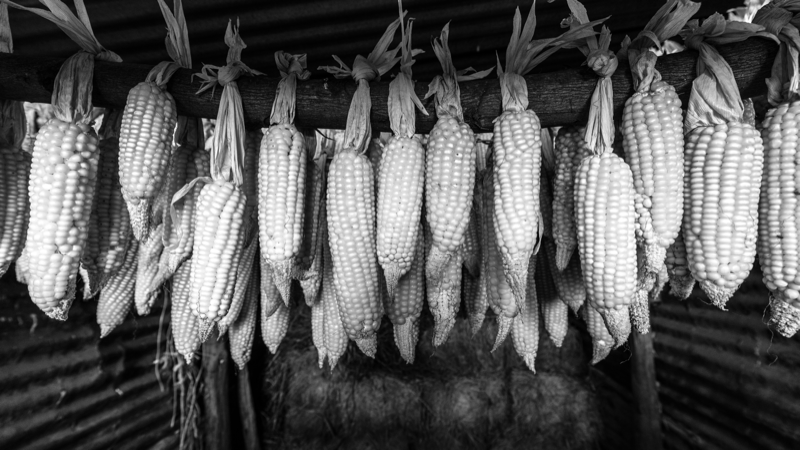
\includegraphics{../assets/farm_02.png}

\hypertarget{chapter-objectives}{%
\subsection{Chapter Objectives}\label{chapter-objectives}}

\begin{itemize}
\tightlist
\item
  Understand the tradeoffs between yield, climate, and crop phenology.
\item
  Learn to use functions to expedite repetative analysis
\item
  Develop a very simple ecohydrological model of soil water availability
\item
  Explore how rainfall seasonality affects the dynamics of soil water
  availability in annual crop systems
\item
  Learn how to run ensembles of simulations and aggregate output
\item
  Examine how planting date and crop choice alter average soil moisture
  during the growing season
\end{itemize}

\hypertarget{laikipia-climate}{%
\subsection{Laikipia Climate}\label{laikipia-climate}}

As we've seen, the climate of northern Kenya is marked by pronounced
rainfall variability. In addition, there is very little variation in
temperature and solar radiation. The graphs below provide long-term
monthly patterns of both temperature and rainfall, which emphasize the
dominat role that temporal variation in rainfall plays in governing the
climate of this system.

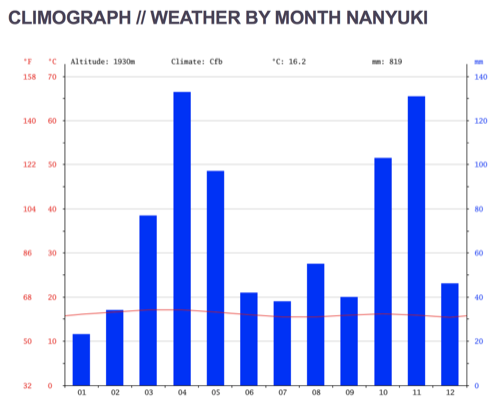
\includegraphics{../assets/nanyuki_rainfall.png}

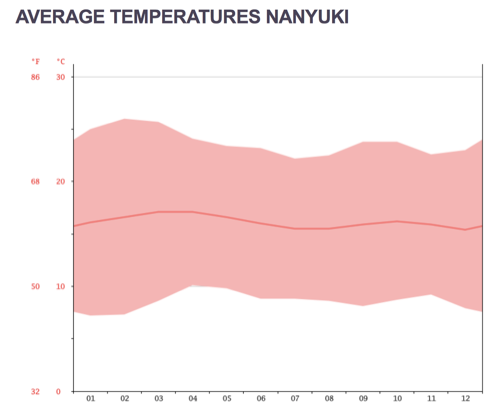
\includegraphics{../assets/nanyuki_temperature.png}

\hypertarget{climate-variability-and-decision-making}{%
\subsection{Climate variability and decision
making}\label{climate-variability-and-decision-making}}

Given the variation in rainfall both within and between years, it is
reasonable to wonder what timing of planting is optimal for ensuring the
success of maize, which is the main crop in this region. In addition,
farmers must make decisions about what variety of maize to plant.

\hypertarget{crop-choice}{%
\subsubsection{Crop Choice}\label{crop-choice}}

Decisions about what type of maize to plant break down along two axes:
Early harvesting varieties vs.~Late harvest varieties, and Local
varieties vs.~Hybrid varieties.

Recently, hybrid varieties designed specifically for the dry conditions
of many Kenyan agricultural zones have started to become available. For
example, here's a
\href{https://basis.ucdavis.edu/news/one-change-hybrid-seeds-could-boost-maize-productivity-western-kenya}{report}
based on work at UC Davis on development of Kenya-specific hybrid maize
varieties that shows great promise. That being said, hybrid varieties
require farmers to purchase seeds annually, rather than saving seeds
from the prior year's harvest which creates a cost burden on smallholder
farmers. While it is likely that - just as in US agriculture - hybrid
and even GMO varieties of maize will come to dominate Kenyan
agrticulture in the coming decades, household farms will remain
dependent on local seeds. Regardless, the interaction between economic
and agronomic tradeoffs is too complex for our excercise, so we will
focus on the first decision - choosing between fast-maturing varieties
that produce lower yields vs.~slower-maturing varities that have higher
yields.

We can investigate the relationship between \texttt{yield} and
\texttt{days\ to\ maturity} using some data on hybrid maize varieties
used in Kenya. Eventhough we will be focusing on local maize varieties
which have lower yields overall than any hybrid variety, we can assume
any relationship seen between \texttt{yield} and
\texttt{days\ to\ maturity} in hybrid maize is similar for local maize.

\hypertarget{getting-started}{%
\subsection{Getting started}\label{getting-started}}

As usual, we need to load pands, our plotting libraries, and remind
jupyter to render our plots into our notebooks.

    \begin{Verbatim}[commandchars=\\\{\}]
{\color{incolor}In [{\color{incolor}15}]:} \PY{k+kn}{import} \PY{n+nn}{pandas} \PY{k}{as} \PY{n+nn}{pd}
         \PY{k+kn}{import} \PY{n+nn}{matplotlib}\PY{n+nn}{.}\PY{n+nn}{pyplot} \PY{k}{as} \PY{n+nn}{plt}
         \PY{o}{\PYZpc{}}\PY{k}{matplotlib} inline
\end{Verbatim}


    \begin{Verbatim}[commandchars=\\\{\}]
{\color{incolor}In [{\color{incolor}16}]:} \PY{n}{hybrid\PYZus{}data} \PY{o}{=} \PY{n}{pd}\PY{o}{.}\PY{n}{read\PYZus{}csv}\PY{p}{(}\PY{l+s+s1}{\PYZsq{}}\PY{l+s+s1}{../data/hybrid\PYZus{}yields.csv}\PY{l+s+s1}{\PYZsq{}}\PY{p}{)}
         \PY{n}{hybrid\PYZus{}data}
\end{Verbatim}


\begin{Verbatim}[commandchars=\\\{\}]
{\color{outcolor}Out[{\color{outcolor}16}]:}     Unnamed: 0             VARIETY ALTITUDE  RANGE (M)  yield (kg/ha)  \textbackslash{}
         0            0               H6213           1700-2100         4680.0   
         1            1               H6212           1700-2100         4680.0   
         2            2               H6210           1700-2100         4500.0   
         3            3               H9401           1700-2100         4320.0   
         4            4                H629           1700-2400         4320.0   
         5            5                H628           1500-2100         4140.0   
         6            6                H627           1500-2100         3960.0   
         7            7                H626           1500-2100         3780.0   
         8            8                H625           1500-2100         3600.0   
         9            9                H614           1500-2100         3420.0   
         10          10                H624           1000-1800         2880.0   
         11          11                H623           1000-1800         2520.0   
         12          12                H516           1000-1800         2520.0   
         13          13                H515           1000-1800         2340.0   
         14          14                H513           1000-1800         2160.0   
         15          15                H511           1000-1800         2070.0   
         16          16                 PH4            0 – 1200         1800.0   
         17          17                 PH1            0 – 1200         1350.0   
         18          18                DH01            800-1200         1350.0   
         19          19                DH02          800 – 1200         1350.0   
         20          20                DH03          800 – 1200         1350.0   
         21          21                DH04          800 – 1200         1710.0   
         22          22  Katumani Composite           1000-1900         1350.0   
         23          23                DLC1           1000-1900         1170.0   
         
             days\_to\_maturity  
         0              175.0  
         1              175.0  
         2              175.0  
         3              175.0  
         4              175.0  
         5              165.0  
         6              165.0  
         7              165.0  
         8              165.0  
         9              175.0  
         10             160.0  
         11             165.0  
         12             120.0  
         13             135.0  
         14             125.0  
         15             125.0  
         16             105.0  
         17              97.5  
         18             110.0  
         19             110.0  
         20             110.0  
         21             110.0  
         22              97.5  
         23              97.5  
\end{Verbatim}
            
    We have 23 different hybrid varieties, with data on the \emph{maximum}
\texttt{yield\ (kg/ha)} and \texttt{days\_to\_maturity} for each
variety. Let's see if there's a relationship between these two
variables:

    \begin{Verbatim}[commandchars=\\\{\}]
{\color{incolor}In [{\color{incolor}17}]:} \PY{n}{hybrid\PYZus{}data}\PY{o}{.}\PY{n}{plot}\PY{o}{.}\PY{n}{scatter}\PY{p}{(}\PY{n}{x}\PY{o}{=}\PY{l+s+s1}{\PYZsq{}}\PY{l+s+s1}{days\PYZus{}to\PYZus{}maturity}\PY{l+s+s1}{\PYZsq{}}\PY{p}{,} \PY{n}{y}\PY{o}{=}\PY{l+s+s1}{\PYZsq{}}\PY{l+s+s1}{yield (kg/ha)}\PY{l+s+s1}{\PYZsq{}}\PY{p}{)}
\end{Verbatim}


\begin{Verbatim}[commandchars=\\\{\}]
{\color{outcolor}Out[{\color{outcolor}17}]:} <matplotlib.axes.\_subplots.AxesSubplot at 0x11fd98860>
\end{Verbatim}
            
    \begin{center}
    \adjustimage{max size={0.9\linewidth}{0.9\paperheight}}{output_4_1.png}
    \end{center}
    { \hspace*{\fill} \\}
    
    That's a pretty clear linear relationship, which isn't totally
unexpected; it stands to reason that annual crops that grow for a longer
period will also yield more at harvest time.

✏️ DIY Code: Use the tools and functions from Chapter 2's curve-fitting
excercise to determine the best-fit linear relationship between these
data and the \(r^2\) value.

    \begin{Verbatim}[commandchars=\\\{\}]
{\color{incolor}In [{\color{incolor}18}]:} \PY{c+c1}{\PYZsh{} This cell intentionally left blank [OPTIONAL]}
\end{Verbatim}


    \hypertarget{planting-date}{%
\subsubsection{Planting Date}\label{planting-date}}

Farmers have to choose planting dates in anticipation of there being
adequate rainfall during the subsequent growing period to avoid crop
failure. Despite the promising data in the figure above, which shows
\emph{optimal} yields from hybrid varities of up to 4.5 tons/ha, actual
yields of maize in Kenya are around 1.4-1.6 tons/ha. That number - while
50\% higher than it was only a decade ago - is about 1/3 of the yields
seen in the US Midwest. So even in the absence of crop failure, success
has a lower bound than elsewhere.

\hypertarget{tradoffs-between-yield-planting-date-and-crop-failure}{%
\subsection{Tradoffs between yield, planting date, and crop
failure}\label{tradoffs-between-yield-planting-date-and-crop-failure}}

The remainder of this Chapter will be focused on developing a simple
model that captures the dynamics implicit in the discussion above:

\begin{enumerate}
\def\labelenumi{\arabic{enumi}.}
\tightlist
\item
  Higher yield varieties of maize require longer periods of growth
\item
  Longer periods of growth increase the potention for exposure of crops
  to prolonged drought.
\item
  Prolonged drought increases the probability of crop failure
\item
  The timing of planting determines how these tradeoffs will play out.
\end{enumerate}

Let's take each of these topics in order:

\hypertarget{tradeoffs-between-yield-and-days-to-maturity}{%
\subsubsection{1. Tradeoffs between yield and days to
maturity}\label{tradeoffs-between-yield-and-days-to-maturity}}

Just in case you didn't actually calculate the regression line between
\texttt{yield\ (kg/ha)} and \texttt{days\_to\_maturity} 😉, we can
eyeball the figure, and estimate the slope of the line to be about
\texttt{40:1}, so that each additional day of maturity increases yield
by 40 kg/ha.

\hypertarget{tradoffs-between-days-to-maturity-and-exposure-to-climate-variability}{%
\subsubsection{2. Tradoffs between days to maturity and exposure to
climate
variability}\label{tradoffs-between-days-to-maturity-and-exposure-to-climate-variability}}

This tradeoff is harder to quantify. Instead, we will model the
interaction between days to maturity and crop failure. Our strategy will
be to examine a very field-scale water balance that looks only at
relative water availability {[}mm/mm{]}, \(s\), daily rainfall, \(R\)
{[}mm/day{]}, and daily water demand, which we will characterize as
reference evapotranspiration, \(ET_0\) {[}mm/day{]}. Because temperature
is relatively constant, we will assume that \(ET_0\) is constant.
Therefore our water balance is simply:

\[ \frac{dS}{dt} = R(t) - ET_0 \]

This formulation ignores many important processes related to soil water
storage and plant response to drought. As defined, it is essentially a
cumulative dryness index; during periods of the season when
\(\sum_t R(t) > t \times ET_0\), there will accumulation of water in the
soil. During periods when \(\sum_t R(t) < t \times ET_0\), the soil will
dry out.

Because the amount of plant available water in the soil in bounded
between zero and some maximum, we add an additional parameter,
\(S_{max}\), which is the maximum amount of water \texttt{{[}mm{]}} that
can be stored in the root zone. Now our model looks like this:

\[
\begin{eqnarray}
    \frac{dS}{dt} &=& R(t) - ET_0 & if & (0 \leq S \leq S_{max}) \\
    & & & else; \\
    \frac{dS}{dt} &=& 0 
\end{eqnarray}       
\]

Assuming a typical value of porosity is 0.4 and soil depth is 500 mm
(0.5 meters), the value of \(S_{max}\) is 200, here is what our model
looks like in python:

\begin{Shaded}
\begin{Highlighting}[]
\NormalTok{n }\OperatorTok{=} \FloatTok{0.4}  \CommentTok{# Porosity, [m3/m3]}
\NormalTok{Zr }\OperatorTok{=} \DecValTok{500} \CommentTok{# Rooting depth [mm]}
\NormalTok{S_max }\OperatorTok{=}\NormalTok{ n}\OperatorTok{*}\NormalTok{Zr    }\CommentTok{# Max soil water storage [mm]}
\NormalTok{S[}\DecValTok{0}\NormalTok{] }\OperatorTok{=} \DecValTok{30}  \CommentTok{# Initial soil water storage [mm]}
\NormalTok{ET_0 }\OperatorTok{=} \FloatTok{6.5} \CommentTok{# Daily reference evapotranspiration [mm]}

\NormalTok{S }\OperatorTok{=}\NormalTok{ np.zeros(}\BuiltInTok{len}\NormalTok{(R)) }\CommentTok{# Pre-allocate the array for S}
\NormalTok{dSdt }\OperatorTok{=}\NormalTok{ np.zeros(}\BuiltInTok{len}\NormalTok{(R))}\CommentTok{# Pre-allocate the array for dSdt}

\ControlFlowTok{for}\NormalTok{ t }\KeywordTok{in} \BuiltInTok{range}\NormalTok{(}\BuiltInTok{len}\NormalTok{(R)):}
\NormalTok{    dSdt[t] }\OperatorTok{=}\NormalTok{ R[t] }\OperatorTok{-}\NormalTok{ ET_0}
\NormalTok{    S[t}\OperatorTok{+}\DecValTok{1}\NormalTok{] }\OperatorTok{=}\NormalTok{ S[t] }\OperatorTok{+}\NormalTok{ dSdt[t]}
    \ControlFlowTok{if}\NormalTok{ S[t}\OperatorTok{+}\DecValTok{1}\NormalTok{] }\OperatorTok{<}\NormalTok{ S_max:}
\NormalTok{        S[t}\OperatorTok{+}\DecValTok{1}\NormalTok{] }\OperatorTok{=}\NormalTok{ S_max}
    \ControlFlowTok{if}\NormalTok{ S[t}\OperatorTok{+}\DecValTok{1}\NormalTok{] }\OperatorTok{<} \DecValTok{0}\NormalTok{:}
\NormalTok{        S[t}\OperatorTok{+}\DecValTok{1}\NormalTok{] }\OperatorTok{=} \DecValTok{0}
\end{Highlighting}
\end{Shaded}

However, before implementing the model, we need to organize our rainfall
simulation code so it is easier to work with.

    I've created a few functions that will speed up our analysis.

\hypertarget{read_data}{%
\paragraph{▶️ read\_data()}\label{read_data}}

This function will read in our CETRAD data file and returns a cleaned up
version using the methods we developed in Chapter 2.

    \begin{Verbatim}[commandchars=\\\{\}]
{\color{incolor}In [{\color{incolor}19}]:} \PY{k}{def} \PY{n+nf}{read\PYZus{}data}\PY{p}{(}\PY{p}{)}\PY{p}{:}
         
             \PY{c+c1}{\PYZsh{} Read in the raw csv data.}
             \PY{n}{df} \PY{o}{=} \PY{n}{pd}\PY{o}{.}\PY{n}{read\PYZus{}csv}\PY{p}{(}\PY{l+s+s2}{\PYZdq{}}\PY{l+s+s2}{../data/CETRAD\PYZus{}rainfall.csv}\PY{l+s+s2}{\PYZdq{}}\PY{p}{)}
         
             \PY{c+c1}{\PYZsh{} Step 1. Convert text strings into datetime objects.}
             \PY{n+nb}{format} \PY{o}{=} \PY{l+s+s1}{\PYZsq{}}\PY{l+s+s1}{\PYZpc{}}\PY{l+s+s1}{m/}\PY{l+s+si}{\PYZpc{}d}\PY{l+s+s1}{/}\PY{l+s+s1}{\PYZpc{}}\PY{l+s+s1}{y}\PY{l+s+s1}{\PYZsq{}}  \PY{c+c1}{\PYZsh{} Column RDate has data in M/D/YY}
             \PY{n}{df}\PY{p}{[}\PY{l+s+s1}{\PYZsq{}}\PY{l+s+s1}{Datetime}\PY{l+s+s1}{\PYZsq{}}\PY{p}{]} \PY{o}{=} \PY{n}{pd}\PY{o}{.}\PY{n}{to\PYZus{}datetime}\PY{p}{(}\PY{n}{df}\PY{p}{[}\PY{l+s+s1}{\PYZsq{}}\PY{l+s+s1}{RDate}\PY{l+s+s1}{\PYZsq{}}\PY{p}{]}\PY{p}{,} \PY{n+nb}{format}\PY{o}{=}\PY{n+nb}{format}\PY{p}{)}  \PY{c+c1}{\PYZsh{} Create a new column of datetime objects using RDate.  \PYZsh{} NOQA}
         
             \PY{c+c1}{\PYZsh{} 2. Step 2. Convert future dates inferred during the conversion back into}
             \PY{c+c1}{\PYZsh{} 20th century dates. Python is a future\PYZhy{}looking programming language, and}
             \PY{c+c1}{\PYZsh{} assumes that 1/1/34 is Jan 1, 2034. We fix this by finding all the dates}
             \PY{c+c1}{\PYZsh{} in the future (dt \PYZgt{} datetime.now()) and removing 100 years from}
             \PY{c+c1}{\PYZsh{} their value. This requires using a relativedelta function, which handles}
             \PY{c+c1}{\PYZsh{} weird stuff like leap years.}
             \PY{n}{df}\PY{p}{[}\PY{l+s+s1}{\PYZsq{}}\PY{l+s+s1}{Datetime}\PY{l+s+s1}{\PYZsq{}}\PY{p}{]} \PY{o}{=} \PY{n}{df}\PY{p}{[}\PY{l+s+s1}{\PYZsq{}}\PY{l+s+s1}{Datetime}\PY{l+s+s1}{\PYZsq{}}\PY{p}{]}\PY{o}{.}\PY{n}{map}\PY{p}{(}
                 \PY{k}{lambda} \PY{n}{dt}\PY{p}{:} \PY{n}{dt}\PY{o}{+}\PY{n}{relativedelta}\PY{p}{(}\PY{n}{years}\PY{o}{=}\PY{o}{\PYZhy{}}\PY{l+m+mi}{100}\PY{p}{)} \PY{k}{if} \PY{n}{dt} \PY{o}{\PYZgt{}} \PY{n}{datetime}\PY{o}{.}\PY{n}{now}\PY{p}{(}\PY{p}{)} \PY{k}{else} \PY{n}{dt}\PY{p}{)}
         
             \PY{c+c1}{\PYZsh{} Step 3. Extract the Year and Month from the Datetime to make}
             \PY{c+c1}{\PYZsh{} aggregation easier.}
             \PY{n}{df}\PY{p}{[}\PY{l+s+s1}{\PYZsq{}}\PY{l+s+s1}{Year}\PY{l+s+s1}{\PYZsq{}}\PY{p}{]} \PY{o}{=} \PY{p}{[}\PY{n}{dt}\PY{o}{.}\PY{n}{year} \PY{k}{for} \PY{n}{dt} \PY{o+ow}{in} \PY{n}{df}\PY{p}{[}\PY{l+s+s1}{\PYZsq{}}\PY{l+s+s1}{Datetime}\PY{l+s+s1}{\PYZsq{}}\PY{p}{]}\PY{p}{]}
             \PY{n}{df}\PY{p}{[}\PY{l+s+s1}{\PYZsq{}}\PY{l+s+s1}{Month}\PY{l+s+s1}{\PYZsq{}}\PY{p}{]} \PY{o}{=} \PY{p}{[}\PY{n}{dt}\PY{o}{.}\PY{n}{month} \PY{k}{for} \PY{n}{dt} \PY{o+ow}{in} \PY{n}{df}\PY{p}{[}\PY{l+s+s1}{\PYZsq{}}\PY{l+s+s1}{Datetime}\PY{l+s+s1}{\PYZsq{}}\PY{p}{]}\PY{p}{]}
         
             \PY{c+c1}{\PYZsh{} Step 4. Use the Datetime values as the index for this dataframe.}
             \PY{n}{df} \PY{o}{=} \PY{n}{df}\PY{o}{.}\PY{n}{set\PYZus{}index}\PY{p}{(}\PY{n}{pd}\PY{o}{.}\PY{n}{DatetimeIndex}\PY{p}{(}\PY{n}{df}\PY{p}{[}\PY{l+s+s1}{\PYZsq{}}\PY{l+s+s1}{Datetime}\PY{l+s+s1}{\PYZsq{}}\PY{p}{]}\PY{p}{)}\PY{p}{)}  \PY{c+c1}{\PYZsh{} Set the Datetime column as the dataframe index \PYZsh{} NOQA}
         
             \PY{c+c1}{\PYZsh{} Step 5.  Delete the old RDate column, which we no longer need.}
             \PY{c+c1}{\PYZsh{} We will keep the Datetime column, in case we need it later.}
             \PY{n}{df} \PY{o}{=} \PY{n}{df}\PY{o}{.}\PY{n}{drop}\PY{p}{(}\PY{p}{[}\PY{l+s+s1}{\PYZsq{}}\PY{l+s+s1}{RDate}\PY{l+s+s1}{\PYZsq{}}\PY{p}{]}\PY{p}{,} \PY{n}{axis}\PY{o}{=}\PY{l+m+mi}{1}\PY{p}{)}
         
             \PY{k}{return} \PY{n}{df}
\end{Verbatim}


    \hypertarget{analyze_rainfall}{%
\paragraph{▶️ analyze\_rainfall()}\label{analyze_rainfall}}

This function will analyze a specific station and returns the raw data,
as well as \(\alpha\) and \(\lambda_r\) values for each month. If
start\_date or end\_date are passed, then they are used to subset the
data to specific years. Otherwise, the entire dataset is returned.

    \begin{Verbatim}[commandchars=\\\{\}]
{\color{incolor}In [{\color{incolor}20}]:} \PY{k}{def} \PY{n+nf}{analyze\PYZus{}rainfall}\PY{p}{(}\PY{n}{station}\PY{o}{=}\PY{l+s+s1}{\PYZsq{}}\PY{l+s+s1}{JACOBSON FARM}\PY{l+s+s1}{\PYZsq{}}\PY{p}{,} \PY{n}{start\PYZus{}year}\PY{o}{=}\PY{k+kc}{None}\PY{p}{,} \PY{n}{end\PYZus{}year}\PY{o}{=}\PY{k+kc}{None}\PY{p}{)}\PY{p}{:}
             \PY{n}{rainfall\PYZus{}data} \PY{o}{=} \PY{n}{read\PYZus{}data}\PY{p}{(}\PY{p}{)}
             \PY{n}{data} \PY{o}{=} \PY{n}{rainfall\PYZus{}data}\PY{p}{[}\PY{p}{[}\PY{n}{station}\PY{p}{,} \PY{l+s+s1}{\PYZsq{}}\PY{l+s+s1}{Month}\PY{l+s+s1}{\PYZsq{}}\PY{p}{,} \PY{l+s+s1}{\PYZsq{}}\PY{l+s+s1}{Year}\PY{l+s+s1}{\PYZsq{}}\PY{p}{,} \PY{l+s+s1}{\PYZsq{}}\PY{l+s+s1}{Datetime}\PY{l+s+s1}{\PYZsq{}}\PY{p}{]}\PY{p}{]}
             \PY{k}{if} \PY{o+ow}{not} \PY{n}{start\PYZus{}year}\PY{p}{:}
                 \PY{n}{start\PYZus{}year} \PY{o}{=} \PY{n+nb}{min}\PY{p}{(}\PY{n}{data}\PY{p}{[}\PY{l+s+s1}{\PYZsq{}}\PY{l+s+s1}{Year}\PY{l+s+s1}{\PYZsq{}}\PY{p}{]}\PY{p}{)}
             \PY{k}{if} \PY{o+ow}{not} \PY{n}{end\PYZus{}year}\PY{p}{:}
                 \PY{n}{end\PYZus{}year} \PY{o}{=} \PY{n+nb}{max}\PY{p}{(}\PY{n}{data}\PY{p}{[}\PY{l+s+s1}{\PYZsq{}}\PY{l+s+s1}{Year}\PY{l+s+s1}{\PYZsq{}}\PY{p}{]}\PY{p}{)}
             \PY{k}{if} \PY{n}{start\PYZus{}year} \PY{o}{\PYZlt{}} \PY{n+nb}{min}\PY{p}{(}\PY{n}{data}\PY{p}{[}\PY{l+s+s1}{\PYZsq{}}\PY{l+s+s1}{Year}\PY{l+s+s1}{\PYZsq{}}\PY{p}{]}\PY{p}{)}\PY{p}{:}
                 \PY{n}{start\PYZus{}year} \PY{o}{=} \PY{n+nb}{min}\PY{p}{(}\PY{n}{data}\PY{p}{[}\PY{l+s+s1}{\PYZsq{}}\PY{l+s+s1}{Year}\PY{l+s+s1}{\PYZsq{}}\PY{p}{]}\PY{p}{)}
             \PY{k}{if} \PY{n}{end\PYZus{}year} \PY{o}{\PYZgt{}} \PY{n+nb}{max}\PY{p}{(}\PY{n}{data}\PY{p}{[}\PY{l+s+s1}{\PYZsq{}}\PY{l+s+s1}{Year}\PY{l+s+s1}{\PYZsq{}}\PY{p}{]}\PY{p}{)}\PY{p}{:}
                 \PY{n}{end\PYZus{}year} \PY{o}{=} \PY{n+nb}{max}\PY{p}{(}\PY{n}{data}\PY{p}{[}\PY{l+s+s1}{\PYZsq{}}\PY{l+s+s1}{Year}\PY{l+s+s1}{\PYZsq{}}\PY{p}{]}\PY{p}{)}
             \PY{n}{data} \PY{o}{=} \PY{n}{data}\PY{o}{.}\PY{n}{loc}\PY{p}{[}\PY{p}{(}\PY{n}{data}\PY{p}{[}\PY{l+s+s1}{\PYZsq{}}\PY{l+s+s1}{Year}\PY{l+s+s1}{\PYZsq{}}\PY{p}{]} \PY{o}{\PYZgt{}}\PY{o}{=} \PY{n}{start\PYZus{}year}\PY{p}{)} \PY{o}{\PYZam{}} \PY{p}{(}\PY{n}{data}\PY{p}{[}\PY{l+s+s1}{\PYZsq{}}\PY{l+s+s1}{Year}\PY{l+s+s1}{\PYZsq{}}\PY{p}{]} \PY{o}{\PYZlt{}}\PY{o}{=} \PY{n}{end\PYZus{}year}\PY{p}{)}\PY{p}{]}
         
             \PY{c+c1}{\PYZsh{} First, find all the rows in the data where it rained and group by month.}
             \PY{n}{rain\PYZus{}days} \PY{o}{=} \PY{n}{data}\PY{o}{.}\PY{n}{loc}\PY{p}{[}\PY{n}{data}\PY{p}{[}\PY{n}{station}\PY{p}{]} \PY{o}{\PYZgt{}} \PY{l+m+mi}{0}\PY{p}{]}
         
             \PY{c+c1}{\PYZsh{} Find all locations in the data where an observation was made.}
             \PY{n}{all\PYZus{}days} \PY{o}{=} \PY{n}{data}\PY{o}{.}\PY{n}{loc}\PY{p}{[}\PY{n}{data}\PY{p}{[}\PY{n}{station}\PY{p}{]} \PY{o}{\PYZgt{}}\PY{o}{=} \PY{l+m+mi}{0}\PY{p}{]}
         
             \PY{n}{lambda\PYZus{}by\PYZus{}month} \PY{o}{=} \PY{p}{(}
                 \PY{n}{rain\PYZus{}days}\PY{o}{.}\PY{n}{groupby}\PY{p}{(}\PY{l+s+s1}{\PYZsq{}}\PY{l+s+s1}{Month}\PY{l+s+s1}{\PYZsq{}}\PY{p}{)}\PY{p}{[}\PY{n}{station}\PY{p}{]}\PY{o}{.}\PY{n}{count}\PY{p}{(}\PY{p}{)} \PY{o}{/}
                 \PY{n}{all\PYZus{}days}\PY{o}{.}\PY{n}{groupby}\PY{p}{(}\PY{l+s+s1}{\PYZsq{}}\PY{l+s+s1}{Month}\PY{l+s+s1}{\PYZsq{}}\PY{p}{)}\PY{p}{[}\PY{n}{station}\PY{p}{]}\PY{o}{.}\PY{n}{count}\PY{p}{(}\PY{p}{)}
             \PY{p}{)}
         
             \PY{n}{alpha} \PY{o}{=} \PY{n}{rain\PYZus{}days}\PY{p}{[}\PY{n}{station}\PY{p}{]}\PY{o}{.}\PY{n}{mean}\PY{p}{(}\PY{p}{)}
         
             \PY{k}{return} \PY{n}{alpha}\PY{p}{,} \PY{n}{lambda\PYZus{}by\PYZus{}month}\PY{p}{,} \PY{n}{data}
\end{Verbatim}


    \hypertarget{seasonal_lambdas}{%
\paragraph{▶️ seasonal\_lambdas()}\label{seasonal_lambdas}}

Generates \(\lambda_r\) values for each day in a growing season given a
planting\_date and an array of 12 \(\lambda_r\) values
(lambda\_by\_month).

    \begin{Verbatim}[commandchars=\\\{\}]
{\color{incolor}In [{\color{incolor}1}]:} \PY{k+kn}{from} \PY{n+nn}{datetime} \PY{k}{import} \PY{n}{datetime}\PY{p}{,} \PY{n}{timedelta}
        \PY{k}{def} \PY{n+nf}{seasonal\PYZus{}lambdas}\PY{p}{(}\PY{n}{lambda\PYZus{}by\PYZus{}month}\PY{p}{,} \PY{n}{planting\PYZus{}date}\PY{o}{=}\PY{n}{datetime}\PY{o}{.}\PY{n}{now}\PY{p}{(}\PY{p}{)}\PY{p}{,} \PY{n}{days\PYZus{}to\PYZus{}maturity}\PY{o}{=}\PY{l+m+mi}{150}\PY{p}{)}\PY{p}{:}
            \PY{l+s+sd}{\PYZdq{}\PYZdq{}\PYZdq{} Generates daily values of lambda\PYZus{}r for a growing season. }
        \PY{l+s+sd}{    }
        \PY{l+s+sd}{    Usage: seasonal\PYZus{}lambdas(lambda\PYZus{}by\PYZus{}month, planting\PYZus{}date=datetime.now(), days\PYZus{}to\PYZus{}maturity=150)}
        \PY{l+s+sd}{    }
        \PY{l+s+sd}{    Arguments:}
        \PY{l+s+sd}{        lambdas\PYZus{}by\PYZus{}month: an array of 12 values of lambda\PYZus{}r, one for each month.}
        \PY{l+s+sd}{        planting\PYZus{}date: The datetime of planting. Default is today.}
        \PY{l+s+sd}{        days\PYZus{}to\PYZus{}maturity: The length of the growing season}
        \PY{l+s+sd}{    \PYZdq{}\PYZdq{}\PYZdq{}}
            \PY{n}{start\PYZus{}date} \PY{o}{=} \PY{n}{planting\PYZus{}date}
            \PY{n}{end\PYZus{}date} \PY{o}{=} \PY{n}{planting\PYZus{}date} \PY{o}{+} \PY{n}{timedelta}\PY{p}{(}\PY{n}{days}\PY{o}{=}\PY{n}{days\PYZus{}to\PYZus{}maturity}\PY{p}{)}
            \PY{n}{datetimes} \PY{o}{=} \PY{n}{np}\PY{o}{.}\PY{n}{arange}\PY{p}{(}
                \PY{n}{start\PYZus{}date}\PY{p}{,} \PY{n}{end\PYZus{}date}\PY{p}{,} \PY{n}{timedelta}\PY{p}{(}\PY{n}{days}\PY{o}{=}\PY{l+m+mi}{1}\PY{p}{)}\PY{p}{)}\PY{o}{.}\PY{n}{astype}\PY{p}{(}\PY{n}{datetime}\PY{p}{)}
            \PY{n}{month\PYZus{}value\PYZus{}by\PYZus{}day} \PY{o}{=} \PY{n}{np}\PY{o}{.}\PY{n}{array}\PY{p}{(}\PY{p}{[}\PY{n}{datetime}\PY{o}{.}\PY{n}{month} \PY{k}{for} \PY{n}{datetime} \PY{o+ow}{in} \PY{n}{datetimes}\PY{p}{]}\PY{p}{)}
            \PY{n}{lambda\PYZus{}values} \PY{o}{=} \PY{n}{np}\PY{o}{.}\PY{n}{array}\PY{p}{(}\PY{p}{[}\PY{n}{lambda\PYZus{}by\PYZus{}month}\PY{p}{[}\PY{n}{i}\PY{p}{]} \PY{k}{for} \PY{n}{i} \PY{o+ow}{in} \PY{n}{month\PYZus{}value\PYZus{}by\PYZus{}day}\PY{p}{]}\PY{p}{)}
            \PY{k}{return} \PY{n}{lambda\PYZus{}values}\PY{p}{,} \PY{n}{datetimes}
\end{Verbatim}


    \hypertarget{simulate_rainfall}{%
\paragraph{▶️ simulate\_rainfall()}\label{simulate_rainfall}}

Generates a simulation of a season of rainfall. Uses a planting date
(which must be passed as a DateTime object, as well as a lenght of the
growing season (days\_to\_maturity), which have default values of now()
and 150, respectively. Requires passing in an array of 12 \(\lambda_r\)
values (lambda\_by\_month), and a single value of \(\alpha\) (alpha).
Returns a time series of daily rainfall in mm (simulated rainfall).

    \begin{Verbatim}[commandchars=\\\{\}]
{\color{incolor}In [{\color{incolor}2}]:} \PY{k}{def} \PY{n+nf}{simulate\PYZus{}rainfall}\PY{p}{(}\PY{n}{lambda\PYZus{}by\PYZus{}month}\PY{p}{,} \PY{n}{alpha}\PY{p}{,} \PY{n}{planting\PYZus{}date}\PY{o}{=}\PY{n}{datetime}\PY{o}{.}\PY{n}{now}\PY{p}{(}\PY{p}{)}\PY{p}{,} \PY{n}{days\PYZus{}to\PYZus{}maturity}\PY{o}{=}\PY{l+m+mi}{150}\PY{p}{,} \PY{n}{n\PYZus{}seasons}\PY{o}{=}\PY{l+m+mi}{1}\PY{p}{)}\PY{p}{:}
            \PY{l+s+sd}{\PYZdq{}\PYZdq{}\PYZdq{} Simulates a season of rainfall.}
        
        \PY{l+s+sd}{    Usage:}
        
        \PY{l+s+sd}{    simulate\PYZus{}rainfall(}
        \PY{l+s+sd}{        planting\PYZus{}date=datetime, days\PYZus{}to\PYZus{}maturity,}
        \PY{l+s+sd}{        lambda\PYZus{}values, alpha\PYZus{}values}
        \PY{l+s+sd}{    )}
        
        \PY{l+s+sd}{    Arguments:}
        \PY{l+s+sd}{        \PYZhy{} planting\PYZus{}date = datetime object specifying month/day of planting.}
        \PY{l+s+sd}{        \PYZhy{} days\PYZus{}to\PYZus{}maturity \PYZhy{} integer number of days until crop is mature}
        \PY{l+s+sd}{        \PYZhy{} lambda\PYZus{}values \PYZhy{} array of 12 lambda values; one for each month}
        \PY{l+s+sd}{        \PYZhy{} alpha value \PYZhy{} a constant average storm depth}
        
        \PY{l+s+sd}{    \PYZdq{}\PYZdq{}\PYZdq{}}
            \PY{n}{lambda\PYZus{}values}\PY{p}{,} \PY{n}{datetimes} \PY{o}{=} \PY{n}{seasonal\PYZus{}lambdas}\PY{p}{(}\PY{n}{lambda\PYZus{}by\PYZus{}month}\PY{p}{,} \PY{n}{planting\PYZus{}date}\PY{p}{,} \PY{n}{days\PYZus{}to\PYZus{}maturity}\PY{p}{)}
            \PY{n}{size} \PY{o}{=} \PY{p}{[}\PY{n}{n\PYZus{}seasons}\PY{p}{,} \PY{n+nb}{len}\PY{p}{(}\PY{n}{lambda\PYZus{}values}\PY{p}{)}\PY{p}{]}
            \PY{n}{simulated\PYZus{}rainy\PYZus{}days} \PY{o}{=} \PY{p}{(}\PY{n}{np}\PY{o}{.}\PY{n}{random}\PY{o}{.}\PY{n}{uniform}\PY{p}{(}
                \PY{n}{low}\PY{o}{=}\PY{l+m+mi}{0}\PY{p}{,} \PY{n}{high}\PY{o}{=}\PY{l+m+mi}{1}\PY{p}{,} \PY{n}{size}\PY{o}{=}\PY{n}{size}\PY{p}{)} \PY{o}{\PYZlt{}}\PY{o}{=} \PY{n}{lambda\PYZus{}values}\PY{p}{)}\PY{o}{.}\PY{n}{astype}\PY{p}{(}\PY{n+nb}{int}\PY{p}{)}
            \PY{n}{simulated\PYZus{}rainfall\PYZus{}values} \PY{o}{=} \PY{n}{np}\PY{o}{.}\PY{n}{random}\PY{o}{.}\PY{n}{exponential}\PY{p}{(}\PY{n}{scale}\PY{o}{=}\PY{n}{alpha}\PY{p}{,} \PY{n}{size}\PY{o}{=}\PY{n}{size}\PY{p}{)}
            \PY{n}{simulated\PYZus{}rainfall} \PY{o}{=} \PY{n}{simulated\PYZus{}rainy\PYZus{}days} \PY{o}{*} \PY{n}{simulated\PYZus{}rainfall\PYZus{}values}
            \PY{k}{return} \PY{n}{simulated\PYZus{}rainfall}\PY{o}{.}\PY{n}{squeeze}\PY{p}{(}\PY{p}{)}\PY{p}{,} \PY{n}{datetimes}
            \PY{c+c1}{\PYZsh{} df =  pd.DataFrame(simulated\PYZus{}rainfall).transpose()}
            \PY{c+c1}{\PYZsh{} return df}
\end{Verbatim}


    \hypertarget{running-the-rainfall-model}{%
\paragraph{▶️ Running the rainfall
model}\label{running-the-rainfall-model}}

We can run the entire rainfall model using this sequence of commands:

\begin{Shaded}
\begin{Highlighting}[]
\NormalTok{    alpha, lambda_by_month, data }\OperatorTok{=}\NormalTok{ analyze_rainfall(station}\OperatorTok{=}\StringTok{'JACOBSON FARM'}\NormalTok{)}
\NormalTok{    R }\OperatorTok{=}\NormalTok{ simulate_rainfall(lambda_by_month, alpha)}
\end{Highlighting}
\end{Shaded}

✏️ DIY Code: Use the model functions to generate rainfall for 30 years
for the station RUMURUTI (NRM).

    \begin{Verbatim}[commandchars=\\\{\}]
{\color{incolor}In [{\color{incolor} }]:} \PY{c+c1}{\PYZsh{} This cell intentionally left blank}
\end{Verbatim}


    \begin{Verbatim}[commandchars=\\\{\}]
{\color{incolor}In [{\color{incolor} }]:} \PY{n}{alpha}\PY{p}{,} \PY{n}{lambda\PYZus{}by\PYZus{}month}\PY{p}{,} \PY{n}{data} \PY{o}{=} \PY{n}{analyze\PYZus{}rainfall}\PY{p}{(}\PY{n}{station}\PY{o}{=}\PY{l+s+s1}{\PYZsq{}}\PY{l+s+s1}{JACOBSON FARM}\PY{l+s+s1}{\PYZsq{}}\PY{p}{)}
        \PY{n}{R}\PY{p}{,} \PY{n}{dt} \PY{o}{=} \PY{n}{simulate\PYZus{}rainfall}\PY{p}{(}\PY{n}{lambda\PYZus{}by\PYZus{}month}\PY{p}{,} \PY{n}{alpha}\PY{p}{,} \PY{n}{planting\PYZus{}date}\PY{o}{=}\PY{n}{datetime}\PY{p}{(}\PY{n}{year}\PY{o}{=}\PY{l+m+mi}{2018}\PY{p}{,}\PY{n}{month}\PY{o}{=}\PY{l+m+mi}{12}\PY{p}{,}\PY{n}{day}\PY{o}{=}\PY{l+m+mi}{1}\PY{p}{)}\PY{p}{)}
\end{Verbatim}


    \hypertarget{coding-up-the-ecohydrological-model}{%
\subsection{Coding up the ecohydrological
model}\label{coding-up-the-ecohydrological-model}}

Now that we have a 2-line method for generating rainfall, let's
implement our model. Here's the code from above, ready to run.

    \begin{Verbatim}[commandchars=\\\{\}]
{\color{incolor}In [{\color{incolor} }]:} \PY{k}{def} \PY{n+nf}{run\PYZus{}model}\PY{p}{(}\PY{n}{R}\PY{p}{,}\PY{n}{Zr}\PY{o}{=}\PY{l+m+mi}{500}\PY{p}{,}\PY{n}{ET\PYZus{}0}\PY{o}{=}\PY{l+m+mf}{3.5}\PY{p}{,}\PY{n}{S\PYZus{}0}\PY{o}{=}\PY{l+m+mi}{30}\PY{p}{,}\PY{n}{n}\PY{o}{=}\PY{l+m+mf}{0.4}\PY{p}{,}\PY{p}{)}\PY{p}{:}
            \PY{l+s+sd}{\PYZdq{}\PYZdq{}\PYZdq{} Runs a simple model with constant ET\PYZus{}o. }
        \PY{l+s+sd}{    }
        \PY{l+s+sd}{    Usage: run\PYZus{}model(R,Zr=500,ET\PYZus{}0=6.5,S\PYZus{}0=30,n=0.4,)}
        \PY{l+s+sd}{        Note: R must be a single\PYZhy{}dimension array}
        \PY{l+s+sd}{        n = 0.4  \PYZsh{} Porosity, [m3/m3]}
        \PY{l+s+sd}{        Zr = 500 \PYZsh{} Rooting depth [mm]}
        \PY{l+s+sd}{        ET\PYZus{}0 = 6.5 \PYZsh{} Daily reference evapotranspiration [mm]}
        \PY{l+s+sd}{    \PYZdq{}\PYZdq{}\PYZdq{}}
            \PY{n}{S\PYZus{}max} \PY{o}{=} \PY{n}{n}\PY{o}{*}\PY{n}{Zr}    \PY{c+c1}{\PYZsh{} Max soil water storage [mm]}
            
            \PY{n}{S} \PY{o}{=} \PY{n}{np}\PY{o}{.}\PY{n}{zeros}\PY{p}{(}\PY{n+nb}{len}\PY{p}{(}\PY{n}{R}\PY{p}{)}\PY{p}{)} \PY{c+c1}{\PYZsh{} Pre\PYZhy{}allocate the array for S}
            \PY{n}{dSdt} \PY{o}{=} \PY{n}{np}\PY{o}{.}\PY{n}{zeros}\PY{p}{(}\PY{n+nb}{len}\PY{p}{(}\PY{n}{R}\PY{p}{)}\PY{p}{)}\PY{c+c1}{\PYZsh{} Pre\PYZhy{}allocate the array for dSdt}
        
            \PY{n}{S}\PY{p}{[}\PY{l+m+mi}{0}\PY{p}{]} \PY{o}{=} \PY{l+m+mi}{16}  \PY{c+c1}{\PYZsh{} Initial soil water storage [mm]}
        
            \PY{k}{for} \PY{n}{t} \PY{o+ow}{in} \PY{n+nb}{range}\PY{p}{(}\PY{n+nb}{len}\PY{p}{(}\PY{n}{R}\PY{p}{)}\PY{p}{)}\PY{p}{:}
                \PY{n}{dSdt}\PY{p}{[}\PY{n}{t}\PY{p}{]} \PY{o}{=} \PY{n}{R}\PY{p}{[}\PY{n}{t}\PY{p}{]} \PY{o}{\PYZhy{}} \PY{n}{ET\PYZus{}0}
                \PY{k}{try}\PY{p}{:} \PY{c+c1}{\PYZsh{} This try block avoids errors from trying to access t+1 on final timestep.}
                    \PY{n}{S}\PY{p}{[}\PY{n}{t}\PY{o}{+}\PY{l+m+mi}{1}\PY{p}{]} \PY{o}{=} \PY{n}{S}\PY{p}{[}\PY{n}{t}\PY{p}{]} \PY{o}{+} \PY{n}{dSdt}\PY{p}{[}\PY{n}{t}\PY{p}{]}
                    \PY{k}{if} \PY{n}{S}\PY{p}{[}\PY{n}{t}\PY{o}{+}\PY{l+m+mi}{1}\PY{p}{]} \PY{o}{\PYZgt{}} \PY{n}{S\PYZus{}max}\PY{p}{:}
                        \PY{n}{S}\PY{p}{[}\PY{n}{t}\PY{o}{+}\PY{l+m+mi}{1}\PY{p}{]} \PY{o}{=} \PY{n}{S\PYZus{}max}
                    \PY{k}{if} \PY{n}{S}\PY{p}{[}\PY{n}{t}\PY{o}{+}\PY{l+m+mi}{1}\PY{p}{]} \PY{o}{\PYZlt{}} \PY{l+m+mi}{0}\PY{p}{:}
                        \PY{n}{S}\PY{p}{[}\PY{n}{t}\PY{o}{+}\PY{l+m+mi}{1}\PY{p}{]} \PY{o}{=} \PY{l+m+mi}{0}
                \PY{k}{except} \PY{n+ne}{IndexError}\PY{p}{:}
                    \PY{k}{return} \PY{p}{\PYZob{}}
                        \PY{l+s+s1}{\PYZsq{}}\PY{l+s+s1}{dSdt}\PY{l+s+s1}{\PYZsq{}}\PY{p}{:} \PY{n}{dSdt}\PY{p}{,}
                        \PY{l+s+s1}{\PYZsq{}}\PY{l+s+s1}{S}\PY{l+s+s1}{\PYZsq{}}\PY{p}{:} \PY{n}{S}\PY{p}{,}
                        \PY{l+s+s1}{\PYZsq{}}\PY{l+s+s1}{R}\PY{l+s+s1}{\PYZsq{}}\PY{p}{:} \PY{n}{R}\PY{p}{,}
                        \PY{l+s+s1}{\PYZsq{}}\PY{l+s+s1}{ET\PYZus{}0}\PY{l+s+s1}{\PYZsq{}}\PY{p}{:} \PY{n}{ET\PYZus{}0}
                    \PY{p}{\PYZcb{}}
\end{Verbatim}


    \hypertarget{running-the-ecohydrological-model-single-season}{%
\subsubsection{Running the ecohydrological model (single
season)}\label{running-the-ecohydrological-model-single-season}}

To summarize, running the model requires stiching all the code above
into the following four steps:

\begin{enumerate}
\def\labelenumi{\arabic{enumi}.}
\tightlist
\item
  \textbf{Analyze station rainfall data.} This provides the necessary
  \(\lambda_r\) and\(\alpha\) values for implementing the model.
\end{enumerate}

\begin{Shaded}
\begin{Highlighting}[]
\NormalTok{station }\OperatorTok{=} \StringTok{'JACOBSON FARM'}
\NormalTok{alpha, lambda_by_month, rain_data }\OperatorTok{=}\NormalTok{ analyze_rainfall(station}\OperatorTok{=}\StringTok{'JACOBSON FARM'}\NormalTok{)}
\end{Highlighting}
\end{Shaded}

\begin{enumerate}
\def\labelenumi{\arabic{enumi}.}
\setcounter{enumi}{1}
\tightlist
\item
  \textbf{Simulate seasonal rainfall.} This provides a timeseries of
  rainfall based on planting date that we can use in our ecohydrological
  model.
\end{enumerate}

\begin{Shaded}
\begin{Highlighting}[]
\NormalTok{planting_date }\OperatorTok{=}\NormalTok{ datetime(year}\OperatorTok{=}\DecValTok{2018}\NormalTok{, month}\OperatorTok{=}\DecValTok{11}\NormalTok{, day}\OperatorTok{=}\DecValTok{15}\NormalTok{)}
\NormalTok{R, dt }\OperatorTok{=}\NormalTok{ simulate_rainfall(lambda_by_month, alpha, planting_date}\OperatorTok{=}\NormalTok{planting_date)}
\end{Highlighting}
\end{Shaded}

\begin{enumerate}
\def\labelenumi{\arabic{enumi}.}
\setcounter{enumi}{2}
\tightlist
\item
  \textbf{Run the ecohydrological model.} Now that we have our rainfall
  data, we can run the model.
\end{enumerate}

\begin{Shaded}
\begin{Highlighting}[]
\NormalTok{    output }\OperatorTok{=}\NormalTok{ run_model(R)}
\end{Highlighting}
\end{Shaded}

Here's everything all together:

    \begin{Verbatim}[commandchars=\\\{\}]
{\color{incolor}In [{\color{incolor} }]:} \PY{c+c1}{\PYZsh{} Step 1. Analyze station rainfall data.}
        \PY{n}{station} \PY{o}{=} \PY{l+s+s1}{\PYZsq{}}\PY{l+s+s1}{JACOBSON FARM}\PY{l+s+s1}{\PYZsq{}}
        \PY{n}{alpha}\PY{p}{,} \PY{n}{lambda\PYZus{}by\PYZus{}month}\PY{p}{,} \PY{n}{rain\PYZus{}data} \PY{o}{=} \PY{n}{analyze\PYZus{}rainfall}\PY{p}{(}\PY{n}{station}\PY{o}{=}\PY{n}{station}\PY{p}{)}
        
        \PY{c+c1}{\PYZsh{} Step 2. Simulate seasonal rainfall}
        \PY{n}{planting\PYZus{}date} \PY{o}{=} \PY{n}{datetime}\PY{p}{(}\PY{n}{year}\PY{o}{=}\PY{l+m+mi}{2018}\PY{p}{,} \PY{n}{month}\PY{o}{=}\PY{l+m+mi}{11}\PY{p}{,} \PY{n}{day}\PY{o}{=}\PY{l+m+mi}{15}\PY{p}{)}
        \PY{n}{R}\PY{p}{,} \PY{n}{dt} \PY{o}{=} \PY{n}{simulate\PYZus{}rainfall}\PY{p}{(}\PY{n}{lambda\PYZus{}by\PYZus{}month}\PY{p}{,} \PY{n}{alpha}\PY{p}{)}
        
        \PY{c+c1}{\PYZsh{} Step 3. Run the ecohydrological model.}
        \PY{n}{output} \PY{o}{=} \PY{n}{run\PYZus{}model}\PY{p}{(}\PY{n}{R}\PY{p}{)}
        \PY{n}{S} \PY{o}{=} \PY{n}{output}\PY{p}{[}\PY{l+s+s1}{\PYZsq{}}\PY{l+s+s1}{S}\PY{l+s+s1}{\PYZsq{}}\PY{p}{]}
        \PY{n}{dSdt} \PY{o}{=} \PY{n}{output}\PY{p}{[}\PY{l+s+s1}{\PYZsq{}}\PY{l+s+s1}{dSdt}\PY{l+s+s1}{\PYZsq{}}\PY{p}{]}
\end{Verbatim}


    \begin{Verbatim}[commandchars=\\\{\}]
{\color{incolor}In [{\color{incolor} }]:} \PY{n}{plt}\PY{o}{.}\PY{n}{plot}\PY{p}{(}\PY{n}{dt}\PY{p}{,}\PY{n}{S}\PY{p}{)}
        \PY{n}{plt}\PY{o}{.}\PY{n}{title}\PY{p}{(}\PY{l+s+s2}{\PYZdq{}}\PY{l+s+s2}{Total rainfall }\PY{l+s+si}{\PYZob{}rain:6.0f\PYZcb{}}\PY{l+s+s2}{ [mm],  avg. S:}\PY{l+s+si}{\PYZob{}S:6.2f\PYZcb{}}\PY{l+s+s2}{ [mm]}\PY{l+s+s2}{\PYZdq{}}\PY{o}{.}\PY{n}{format}\PY{p}{(}
            \PY{n}{rain}\PY{o}{=}\PY{n+nb}{sum}\PY{p}{(}\PY{n}{R}\PY{p}{)}\PY{p}{,}
            \PY{n}{S}\PY{o}{=}\PY{n}{S}\PY{o}{.}\PY{n}{mean}\PY{p}{(}\PY{p}{)}
        \PY{p}{)}\PY{p}{)}
\end{Verbatim}


    \hypertarget{running-the-ecohydrological-model-multiple-seasons}{%
\subsubsection{Running the ecohydrological model (multiple
seasons)}\label{running-the-ecohydrological-model-multiple-seasons}}

Running the model for multiple seasons requires only a slight
modification to how we collect the output. Instead of a single
dictionary with the output, we create a list of dictionaries, which each
contain output for one simulation. We are also going to include more
variables explicitly in Step 2:

\begin{Shaded}
\begin{Highlighting}[]
\NormalTok{planting_date }\OperatorTok{=}\NormalTok{ datetime(year}\OperatorTok{=}\DecValTok{2018}\NormalTok{, month}\OperatorTok{=}\DecValTok{10}\NormalTok{, day}\OperatorTok{=}\DecValTok{15}\NormalTok{)}
\NormalTok{n_seasons }\OperatorTok{=} \DecValTok{100}
\NormalTok{days_to_maturity }\OperatorTok{=} \DecValTok{150}
\end{Highlighting}
\end{Shaded}

    \begin{Verbatim}[commandchars=\\\{\}]
{\color{incolor}In [{\color{incolor} }]:} \PY{c+c1}{\PYZsh{} Step 1. Analyze station rainfall data.}
        \PY{n}{station} \PY{o}{=} \PY{l+s+s1}{\PYZsq{}}\PY{l+s+s1}{JACOBSON FARM}\PY{l+s+s1}{\PYZsq{}}
        \PY{n}{alpha}\PY{p}{,} \PY{n}{lambda\PYZus{}by\PYZus{}month}\PY{p}{,} \PY{n}{rain\PYZus{}data} \PY{o}{=} \PY{n}{analyze\PYZus{}rainfall}\PY{p}{(}\PY{n}{station}\PY{o}{=}\PY{n}{station}\PY{p}{)}
        
        \PY{c+c1}{\PYZsh{} Step 2. Simulate n seasons of rainfall}
        \PY{k+kn}{from} \PY{n+nn}{datetime} \PY{k}{import} \PY{n}{timedelta}
        
        \PY{n}{planting\PYZus{}date} \PY{o}{=} \PY{n}{datetime}\PY{p}{(}\PY{n}{year}\PY{o}{=}\PY{l+m+mi}{2018}\PY{p}{,} \PY{n}{month}\PY{o}{=}\PY{l+m+mi}{3}\PY{p}{,} \PY{n}{day}\PY{o}{=}\PY{l+m+mi}{15}\PY{p}{)}
        \PY{n}{n\PYZus{}seasons} \PY{o}{=} \PY{l+m+mi}{100}
        \PY{n}{days\PYZus{}to\PYZus{}maturity} \PY{o}{=} \PY{l+m+mi}{150}
        
        \PY{n}{R}\PY{p}{,} \PY{n}{dt} \PY{o}{=} \PY{n}{simulate\PYZus{}rainfall}\PY{p}{(}\PY{n}{lambda\PYZus{}by\PYZus{}month}\PY{p}{,} \PY{n}{alpha}\PY{p}{,} \PY{n}{planting\PYZus{}date}\PY{o}{=}\PY{n}{planting\PYZus{}date}\PY{p}{,} \PY{n}{n\PYZus{}seasons}\PY{o}{=}\PY{n}{n\PYZus{}seasons}\PY{p}{)}
        
        \PY{c+c1}{\PYZsh{} Step 3. Run the ecohydrological model.}
        \PY{n}{output} \PY{o}{=} \PY{p}{[}\PY{p}{]}
        \PY{n}{S} \PY{o}{=} \PY{p}{[}\PY{p}{]}
        \PY{n}{dSdt} \PY{o}{=} \PY{p}{[}\PY{p}{]}
        \PY{k}{for} \PY{n}{r} \PY{o+ow}{in} \PY{n}{R}\PY{p}{:}
            \PY{n}{output} \PY{o}{=} \PY{p}{(}\PY{n}{run\PYZus{}model}\PY{p}{(}\PY{n}{r}\PY{p}{)}\PY{p}{)}
            \PY{n}{S}\PY{o}{.}\PY{n}{append}\PY{p}{(}\PY{n}{output}\PY{p}{[}\PY{l+s+s1}{\PYZsq{}}\PY{l+s+s1}{S}\PY{l+s+s1}{\PYZsq{}}\PY{p}{]}\PY{p}{)}
            \PY{n}{dSdt}\PY{o}{.}\PY{n}{append}\PY{p}{(}\PY{n}{output}\PY{p}{[}\PY{l+s+s1}{\PYZsq{}}\PY{l+s+s1}{dSdt}\PY{l+s+s1}{\PYZsq{}}\PY{p}{]}\PY{p}{)}
        
        \PY{c+c1}{\PYZsh{} It\PYZsq{}s very easy to turn a list of lists into a `DataFrame`}
        \PY{n}{df\PYZus{}S} \PY{o}{=} \PY{n}{pd}\PY{o}{.}\PY{n}{DataFrame}\PY{p}{(}\PY{n}{S}\PY{p}{)}
        \PY{n}{plt}\PY{o}{.}\PY{n}{plot}\PY{p}{(}\PY{n}{dt}\PY{p}{,} \PY{n}{df\PYZus{}S}\PY{o}{.}\PY{n}{mean}\PY{p}{(}\PY{p}{)}\PY{p}{)}
        \PY{n}{plt}\PY{o}{.}\PY{n}{title}\PY{p}{(}\PY{l+s+s2}{\PYZdq{}}\PY{l+s+si}{\PYZob{}date\PYZcb{}}\PY{l+s+s2}{ to }\PY{l+s+si}{\PYZob{}end\PYZcb{}}\PY{l+s+s2}{, n=}\PY{l+s+si}{\PYZob{}n\PYZcb{}}\PY{l+s+s2}{, S\PYZus{}avg=}\PY{l+s+si}{\PYZob{}s:5.2f\PYZcb{}}\PY{l+s+s2}{\PYZdq{}}\PY{o}{.}\PY{n}{format}\PY{p}{(}
            \PY{n}{date}\PY{o}{=}\PY{n}{datetime}\PY{o}{.}\PY{n}{strftime}\PY{p}{(}\PY{n}{planting\PYZus{}date}\PY{p}{,}\PY{l+s+s2}{\PYZdq{}}\PY{l+s+s2}{\PYZpc{}}\PY{l+s+s2}{b }\PY{l+s+si}{\PYZpc{}d}\PY{l+s+s2}{\PYZdq{}}\PY{p}{)}\PY{p}{,}
            \PY{n}{end}\PY{o}{=}\PY{n}{datetime}\PY{o}{.}\PY{n}{strftime}\PY{p}{(}\PY{n}{planting\PYZus{}date}\PY{o}{+}\PY{n}{timedelta}\PY{p}{(}\PY{n}{days}\PY{o}{=}\PY{n}{days\PYZus{}to\PYZus{}maturity}\PY{p}{)}\PY{p}{,}\PY{l+s+s2}{\PYZdq{}}\PY{l+s+s2}{\PYZpc{}}\PY{l+s+s2}{b }\PY{l+s+si}{\PYZpc{}d}\PY{l+s+s2}{\PYZdq{}}\PY{p}{)}\PY{p}{,}
            \PY{n}{n}\PY{o}{=}\PY{n}{n\PYZus{}seasons}\PY{p}{,}
            \PY{n}{s}\PY{o}{=}\PY{n}{df\PYZus{}S}\PY{o}{.}\PY{n}{mean}\PY{p}{(}\PY{p}{)}\PY{o}{.}\PY{n}{mean}\PY{p}{(}\PY{p}{)}\PY{p}{)}\PY{p}{)}
\end{Verbatim}


    \hypertarget{effect-of-planting-date-on-average-soil-water-availability}{%
\subsection{Effect of planting date on average soil water
availability}\label{effect-of-planting-date-on-average-soil-water-availability}}

We can use our model to see how planting date alters the average soil
water availability during the growing season.

We will use a for loop to iterate across planting dates

\begin{Shaded}
\begin{Highlighting}[]
\NormalTok{station }\OperatorTok{=} \StringTok{'JACOBSON FARM'}
\NormalTok{alpha, lambda_by_month, rain_data }\OperatorTok{=}\NormalTok{ analyze_rainfall(station}\OperatorTok{=}\NormalTok{station)}
\NormalTok{n_seasons }\OperatorTok{=} \DecValTok{100}
\NormalTok{days_to_maturity }\OperatorTok{=} \DecValTok{150}

\NormalTok{planting_dates }\OperatorTok{=}\NormalTok{ np.arange(datetime(}\DecValTok{2017}\NormalTok{,}\DecValTok{1}\NormalTok{,}\DecValTok{1}\NormalTok{), datetime(}\DecValTok{2017}\NormalTok{,}\DecValTok{12}\NormalTok{,}\DecValTok{31}\NormalTok{), timedelta(weeks}\OperatorTok{=}\DecValTok{1}\NormalTok{)).astype(datetime)}

\NormalTok{S_avg }\OperatorTok{=}\NormalTok{ []}
\ControlFlowTok{for}\NormalTok{ planting_date }\KeywordTok{in}\NormalTok{ planting_dates:}
\NormalTok{    R, dt }\OperatorTok{=}\NormalTok{ simulate_rainfall(lambda_by_month, alpha, planting_date}\OperatorTok{=}\NormalTok{planting_date, n_seasons}\OperatorTok{=}\NormalTok{n_seasons)}

    \CommentTok{# Step 3. Run the ecohydrological model.}
\NormalTok{    output }\OperatorTok{=}\NormalTok{ []}
\NormalTok{    S }\OperatorTok{=}\NormalTok{ []}
\NormalTok{    dSdt }\OperatorTok{=}\NormalTok{ []}
    \ControlFlowTok{for}\NormalTok{ r }\KeywordTok{in}\NormalTok{ R:}
\NormalTok{        output }\OperatorTok{=}\NormalTok{ (run_model(r))}
\NormalTok{        S.append(output[}\StringTok{'S'}\NormalTok{])}
\NormalTok{        dSdt.append(output[}\StringTok{'dSdt'}\NormalTok{])}
\NormalTok{    df_S }\OperatorTok{=}\NormalTok{ pd.DataFrame(S)}
\NormalTok{    S_avg.append(df_S.mean().mean())}
\end{Highlighting}
\end{Shaded}

    \begin{Verbatim}[commandchars=\\\{\}]
{\color{incolor}In [{\color{incolor} }]:} \PY{n}{station} \PY{o}{=} \PY{l+s+s1}{\PYZsq{}}\PY{l+s+s1}{JACOBSON FARM}\PY{l+s+s1}{\PYZsq{}}
        \PY{n}{alpha}\PY{p}{,} \PY{n}{lambda\PYZus{}by\PYZus{}month}\PY{p}{,} \PY{n}{rain\PYZus{}data} \PY{o}{=} \PY{n}{analyze\PYZus{}rainfall}\PY{p}{(}\PY{n}{station}\PY{o}{=}\PY{n}{station}\PY{p}{)}
        \PY{n}{n\PYZus{}seasons} \PY{o}{=} \PY{l+m+mi}{100}
        \PY{n}{days\PYZus{}to\PYZus{}maturity} \PY{o}{=} \PY{l+m+mi}{150}
        
        \PY{n}{planting\PYZus{}dates} \PY{o}{=} \PY{n}{np}\PY{o}{.}\PY{n}{arange}\PY{p}{(}\PY{n}{datetime}\PY{p}{(}\PY{l+m+mi}{2017}\PY{p}{,}\PY{l+m+mi}{1}\PY{p}{,}\PY{l+m+mi}{1}\PY{p}{)}\PY{p}{,} \PY{n}{datetime}\PY{p}{(}\PY{l+m+mi}{2017}\PY{p}{,}\PY{l+m+mi}{12}\PY{p}{,}\PY{l+m+mi}{31}\PY{p}{)}\PY{p}{,} \PY{n}{timedelta}\PY{p}{(}\PY{n}{weeks}\PY{o}{=}\PY{l+m+mi}{1}\PY{p}{)}\PY{p}{)}\PY{o}{.}\PY{n}{astype}\PY{p}{(}\PY{n}{datetime}\PY{p}{)}
        
        \PY{n}{S\PYZus{}avg} \PY{o}{=} \PY{p}{[}\PY{p}{]}
        \PY{k}{for} \PY{n}{planting\PYZus{}date} \PY{o+ow}{in} \PY{n}{planting\PYZus{}dates}\PY{p}{:}
            \PY{n}{R}\PY{p}{,} \PY{n}{dt} \PY{o}{=} \PY{n}{simulate\PYZus{}rainfall}\PY{p}{(}\PY{n}{lambda\PYZus{}by\PYZus{}month}\PY{p}{,} \PY{n}{alpha}\PY{p}{,} \PY{n}{planting\PYZus{}date}\PY{o}{=}\PY{n}{planting\PYZus{}date}\PY{p}{,} \PY{n}{n\PYZus{}seasons}\PY{o}{=}\PY{n}{n\PYZus{}seasons}\PY{p}{)}
        
            \PY{c+c1}{\PYZsh{} Step 3. Run the ecohydrological model.}
            \PY{n}{output} \PY{o}{=} \PY{p}{[}\PY{p}{]}
            \PY{n}{S} \PY{o}{=} \PY{p}{[}\PY{p}{]}
            \PY{n}{dSdt} \PY{o}{=} \PY{p}{[}\PY{p}{]}
            \PY{k}{for} \PY{n}{r} \PY{o+ow}{in} \PY{n}{R}\PY{p}{:}
                \PY{n}{output} \PY{o}{=} \PY{p}{(}\PY{n}{run\PYZus{}model}\PY{p}{(}\PY{n}{r}\PY{p}{)}\PY{p}{)}
                \PY{n}{S}\PY{o}{.}\PY{n}{append}\PY{p}{(}\PY{n}{output}\PY{p}{[}\PY{l+s+s1}{\PYZsq{}}\PY{l+s+s1}{S}\PY{l+s+s1}{\PYZsq{}}\PY{p}{]}\PY{p}{)}
                \PY{n}{dSdt}\PY{o}{.}\PY{n}{append}\PY{p}{(}\PY{n}{output}\PY{p}{[}\PY{l+s+s1}{\PYZsq{}}\PY{l+s+s1}{dSdt}\PY{l+s+s1}{\PYZsq{}}\PY{p}{]}\PY{p}{)}
            \PY{n}{df\PYZus{}S} \PY{o}{=} \PY{n}{pd}\PY{o}{.}\PY{n}{DataFrame}\PY{p}{(}\PY{n}{S}\PY{p}{)}
            \PY{n}{S\PYZus{}avg}\PY{o}{.}\PY{n}{append}\PY{p}{(}\PY{n}{df\PYZus{}S}\PY{o}{.}\PY{n}{mean}\PY{p}{(}\PY{p}{)}\PY{o}{.}\PY{n}{mean}\PY{p}{(}\PY{p}{)}\PY{p}{)}
        
        \PY{n}{plt}\PY{o}{.}\PY{n}{plot}\PY{p}{(}\PY{n}{planting\PYZus{}dates}\PY{p}{,}\PY{n}{S\PYZus{}avg}\PY{p}{)}
\end{Verbatim}


    It appears that there are two fairly broad periods of moderate water
availability, separated by deep valleys of low water availability. Our
next question is how do planting date and days to maturity interact. We
can examine this by nesting two for loops.

\begin{Shaded}
\begin{Highlighting}[]
\NormalTok{station }\OperatorTok{=} \StringTok{'JACOBSON FARM'}
\NormalTok{alpha, lambda_by_month, rain_data }\OperatorTok{=}\NormalTok{ analyze_rainfall(station}\OperatorTok{=}\NormalTok{station)}
\NormalTok{n_seasons }\OperatorTok{=} \DecValTok{100}
\NormalTok{varieties }\OperatorTok{=}\NormalTok{ [}\DecValTok{120}\NormalTok{, }\DecValTok{180}\NormalTok{]}

\NormalTok{planting_dates }\OperatorTok{=}\NormalTok{ np.arange(datetime(}\DecValTok{2017}\NormalTok{,}\DecValTok{1}\NormalTok{,}\DecValTok{1}\NormalTok{), datetime(}\DecValTok{2017}\NormalTok{,}\DecValTok{12}\NormalTok{,}\DecValTok{31}\NormalTok{), timedelta(weeks}\OperatorTok{=}\DecValTok{1}\NormalTok{)).astype(datetime)}

\NormalTok{S_avg }\OperatorTok{=}\NormalTok{ [[],[]]}

\ControlFlowTok{for}\NormalTok{ planting_date }\KeywordTok{in}\NormalTok{ planting_dates:}
    \ControlFlowTok{for}\NormalTok{ i, days_to_maturity }\KeywordTok{in} \BuiltInTok{enumerate}\NormalTok{(varieties): }
\NormalTok{        R, dt }\OperatorTok{=}\NormalTok{ simulate_rainfall(}
\NormalTok{            lambda_by_month, alpha,}
\NormalTok{            days_to_maturity}\OperatorTok{=}\NormalTok{days_to_maturity,}
\NormalTok{            planting_date}\OperatorTok{=}\NormalTok{planting_date, n_seasons}\OperatorTok{=}\NormalTok{n_seasons)}

        \CommentTok{# Step 3. Run the ecohydrological model.}
\NormalTok{        output }\OperatorTok{=}\NormalTok{ []}
\NormalTok{        S }\OperatorTok{=}\NormalTok{ []}
\NormalTok{        dSdt }\OperatorTok{=}\NormalTok{ []}
        \ControlFlowTok{for}\NormalTok{ r }\KeywordTok{in}\NormalTok{ R:}
\NormalTok{            output }\OperatorTok{=}\NormalTok{ (run_model(r))}
\NormalTok{            S.append(output[}\StringTok{'S'}\NormalTok{])}
\NormalTok{            dSdt.append(output[}\StringTok{'dSdt'}\NormalTok{])}
\NormalTok{        df_S }\OperatorTok{=}\NormalTok{ pd.DataFrame(S)}
\NormalTok{        S_avg[i].append(df_S.mean().mean())}
\end{Highlighting}
\end{Shaded}

    \begin{Verbatim}[commandchars=\\\{\}]
{\color{incolor}In [{\color{incolor} }]:} \PY{n}{station} \PY{o}{=} \PY{l+s+s1}{\PYZsq{}}\PY{l+s+s1}{JACOBSON FARM}\PY{l+s+s1}{\PYZsq{}}
        \PY{n}{alpha}\PY{p}{,} \PY{n}{lambda\PYZus{}by\PYZus{}month}\PY{p}{,} \PY{n}{rain\PYZus{}data} \PY{o}{=} \PY{n}{analyze\PYZus{}rainfall}\PY{p}{(}\PY{n}{station}\PY{o}{=}\PY{n}{station}\PY{p}{)}
        \PY{n}{n\PYZus{}seasons} \PY{o}{=} \PY{l+m+mi}{100}
        \PY{n}{varieties} \PY{o}{=} \PY{p}{[}\PY{l+m+mi}{120}\PY{p}{,} \PY{l+m+mi}{180}\PY{p}{]}
        
        \PY{n}{planting\PYZus{}dates} \PY{o}{=} \PY{n}{np}\PY{o}{.}\PY{n}{arange}\PY{p}{(}\PY{n}{datetime}\PY{p}{(}\PY{l+m+mi}{2017}\PY{p}{,}\PY{l+m+mi}{1}\PY{p}{,}\PY{l+m+mi}{1}\PY{p}{)}\PY{p}{,} \PY{n}{datetime}\PY{p}{(}\PY{l+m+mi}{2017}\PY{p}{,}\PY{l+m+mi}{12}\PY{p}{,}\PY{l+m+mi}{31}\PY{p}{)}\PY{p}{,} \PY{n}{timedelta}\PY{p}{(}\PY{n}{weeks}\PY{o}{=}\PY{l+m+mi}{1}\PY{p}{)}\PY{p}{)}\PY{o}{.}\PY{n}{astype}\PY{p}{(}\PY{n}{datetime}\PY{p}{)}
        
        \PY{n}{S\PYZus{}avg} \PY{o}{=} \PY{p}{[}\PY{p}{[}\PY{p}{]}\PY{p}{,}\PY{p}{[}\PY{p}{]}\PY{p}{]}
        
        \PY{k}{for} \PY{n}{planting\PYZus{}date} \PY{o+ow}{in} \PY{n}{planting\PYZus{}dates}\PY{p}{:}
            \PY{k}{for} \PY{n}{i}\PY{p}{,} \PY{n}{days\PYZus{}to\PYZus{}maturity} \PY{o+ow}{in} \PY{n+nb}{enumerate}\PY{p}{(}\PY{n}{varieties}\PY{p}{)}\PY{p}{:} 
                \PY{n}{R}\PY{p}{,} \PY{n}{dt} \PY{o}{=} \PY{n}{simulate\PYZus{}rainfall}\PY{p}{(}
                    \PY{n}{lambda\PYZus{}by\PYZus{}month}\PY{p}{,} \PY{n}{alpha}\PY{p}{,}
                    \PY{n}{days\PYZus{}to\PYZus{}maturity}\PY{o}{=}\PY{n}{days\PYZus{}to\PYZus{}maturity}\PY{p}{,}
                    \PY{n}{planting\PYZus{}date}\PY{o}{=}\PY{n}{planting\PYZus{}date}\PY{p}{,} \PY{n}{n\PYZus{}seasons}\PY{o}{=}\PY{n}{n\PYZus{}seasons}\PY{p}{)}
        
                \PY{c+c1}{\PYZsh{} Step 3. Run the ecohydrological model.}
                \PY{n}{output} \PY{o}{=} \PY{p}{[}\PY{p}{]}
                \PY{n}{S} \PY{o}{=} \PY{p}{[}\PY{p}{]}
                \PY{n}{dSdt} \PY{o}{=} \PY{p}{[}\PY{p}{]}
                \PY{k}{for} \PY{n}{r} \PY{o+ow}{in} \PY{n}{R}\PY{p}{:}
                    \PY{n}{output} \PY{o}{=} \PY{p}{(}\PY{n}{run\PYZus{}model}\PY{p}{(}\PY{n}{r}\PY{p}{)}\PY{p}{)}
                    \PY{n}{S}\PY{o}{.}\PY{n}{append}\PY{p}{(}\PY{n}{output}\PY{p}{[}\PY{l+s+s1}{\PYZsq{}}\PY{l+s+s1}{S}\PY{l+s+s1}{\PYZsq{}}\PY{p}{]}\PY{p}{)}
                    \PY{n}{dSdt}\PY{o}{.}\PY{n}{append}\PY{p}{(}\PY{n}{output}\PY{p}{[}\PY{l+s+s1}{\PYZsq{}}\PY{l+s+s1}{dSdt}\PY{l+s+s1}{\PYZsq{}}\PY{p}{]}\PY{p}{)}
                \PY{n}{df\PYZus{}S} \PY{o}{=} \PY{n}{pd}\PY{o}{.}\PY{n}{DataFrame}\PY{p}{(}\PY{n}{S}\PY{p}{)}
                \PY{n}{S\PYZus{}avg}\PY{p}{[}\PY{n}{i}\PY{p}{]}\PY{o}{.}\PY{n}{append}\PY{p}{(}\PY{n}{df\PYZus{}S}\PY{o}{.}\PY{n}{mean}\PY{p}{(}\PY{p}{)}\PY{o}{.}\PY{n}{mean}\PY{p}{(}\PY{p}{)}\PY{p}{)}
        
        \PY{n}{df} \PY{o}{=} \PY{n}{pd}\PY{o}{.}\PY{n}{DataFrame}\PY{p}{(}\PY{p}{\PYZob{}}
            \PY{l+s+s1}{\PYZsq{}}\PY{l+s+s1}{x}\PY{l+s+s1}{\PYZsq{}}\PY{p}{:} \PY{n}{planting\PYZus{}dates}\PY{p}{,}
            \PY{l+s+s1}{\PYZsq{}}\PY{l+s+s1}{120\PYZhy{}day}\PY{l+s+s1}{\PYZsq{}}\PY{p}{:} \PY{n}{S\PYZus{}avg}\PY{p}{[}\PY{l+m+mi}{0}\PY{p}{]}\PY{p}{,}
            \PY{l+s+s1}{\PYZsq{}}\PY{l+s+s1}{180\PYZhy{}day}\PY{l+s+s1}{\PYZsq{}}\PY{p}{:} \PY{n}{S\PYZus{}avg}\PY{p}{[}\PY{l+m+mi}{1}\PY{p}{]}
        \PY{p}{\PYZcb{}}\PY{p}{)}
        
        \PY{n}{plt}\PY{o}{.}\PY{n}{plot}\PY{p}{(}
            \PY{l+s+s1}{\PYZsq{}}\PY{l+s+s1}{x}\PY{l+s+s1}{\PYZsq{}}\PY{p}{,} \PY{l+s+s1}{\PYZsq{}}\PY{l+s+s1}{120\PYZhy{}day}\PY{l+s+s1}{\PYZsq{}}\PY{p}{,} \PY{n}{data}\PY{o}{=}\PY{n}{df}\PY{p}{,} \PY{n}{marker}\PY{o}{=}\PY{l+s+s1}{\PYZsq{}}\PY{l+s+s1}{\PYZsq{}}\PY{p}{,} \PY{n}{color}\PY{o}{=}\PY{l+s+s1}{\PYZsq{}}\PY{l+s+s1}{skyblue}\PY{l+s+s1}{\PYZsq{}}\PY{p}{,}
            \PY{n}{label}\PY{o}{=}\PY{l+s+s1}{\PYZsq{}}\PY{l+s+s1}{120\PYZhy{}day variety}\PY{l+s+s1}{\PYZsq{}}\PY{p}{,} \PY{n}{linewidth}\PY{o}{=}\PY{l+m+mi}{2}
        \PY{p}{)}
        \PY{n}{plt}\PY{o}{.}\PY{n}{plot}\PY{p}{(}\PY{l+s+s1}{\PYZsq{}}\PY{l+s+s1}{x}\PY{l+s+s1}{\PYZsq{}}\PY{p}{,} \PY{l+s+s1}{\PYZsq{}}\PY{l+s+s1}{180\PYZhy{}day}\PY{l+s+s1}{\PYZsq{}}\PY{p}{,} \PY{n}{data}\PY{o}{=}\PY{n}{df}\PY{p}{,} \PY{n}{marker}\PY{o}{=}\PY{l+s+s1}{\PYZsq{}}\PY{l+s+s1}{\PYZsq{}}\PY{p}{,} \PY{n}{color}\PY{o}{=}\PY{l+s+s1}{\PYZsq{}}\PY{l+s+s1}{skyblue}\PY{l+s+s1}{\PYZsq{}}\PY{p}{,}
            \PY{n}{label}\PY{o}{=}\PY{l+s+s1}{\PYZsq{}}\PY{l+s+s1}{180\PYZhy{}day variety}\PY{l+s+s1}{\PYZsq{}}\PY{p}{,} \PY{n}{linestyle}\PY{o}{=}\PY{l+s+s1}{\PYZsq{}}\PY{l+s+s1}{dashed}\PY{l+s+s1}{\PYZsq{}}\PY{p}{,} \PY{n}{linewidth}\PY{o}{=}\PY{l+m+mi}{2}
        \PY{p}{)}
        \PY{n}{plt}\PY{o}{.}\PY{n}{legend}\PY{p}{(}\PY{p}{)}
        \PY{n}{plt}\PY{o}{.}\PY{n}{title}\PY{p}{(}\PY{l+s+s1}{\PYZsq{}}\PY{l+s+s1}{Effect of planting date and variety on soil water availability}\PY{l+s+s1}{\PYZsq{}}\PY{p}{)}
\end{Verbatim}


    We see that the variety that matures more quickly has a narrow range of
success, but higher peaks in terms of seasonal water availability.

    \hypertarget{coefficients-of-seasonal-rainfall-variability-across-laikipia}{%
\subsection{Coefficients of Seasonal Rainfall Variability across
Laikipia}\label{coefficients-of-seasonal-rainfall-variability-across-laikipia}}

Analysis from
\href{https://ccafs.cgiar.org/about/people/philip-thornton\#.W4H37S2ZPOQ}{Philip
Thornton} at CCAFS/CGIAR suggests that there are fairly sharp thresholds
in the relationship between rainfall climatology and crop failure. The
following two figures demonstrate this relationship from some of his
previous work.

\href{../assets/crop_failure_vs_rainfall_cv.png}{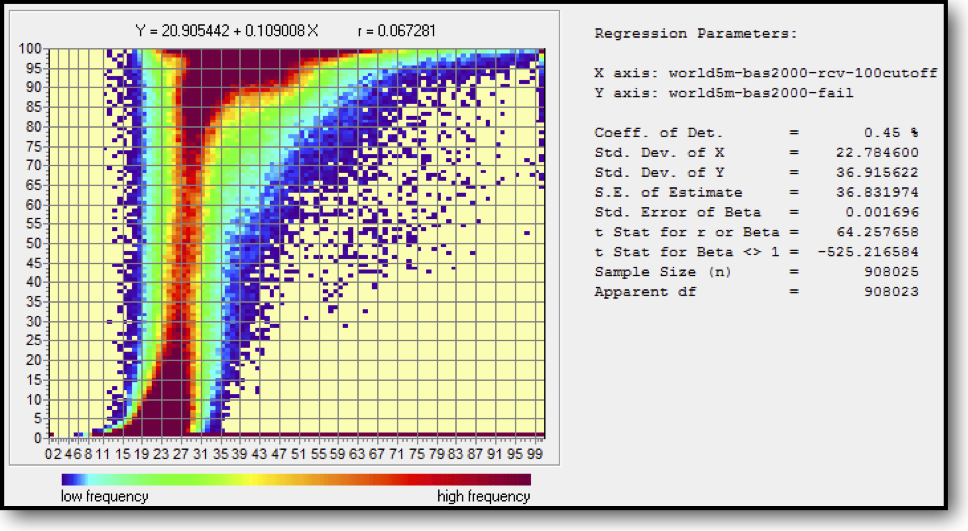
\includegraphics{../assets/crop_failure_vs_rainfall_cv.png}}

\href{../assets/cropping_extent_vs_rainfall_cv.png}{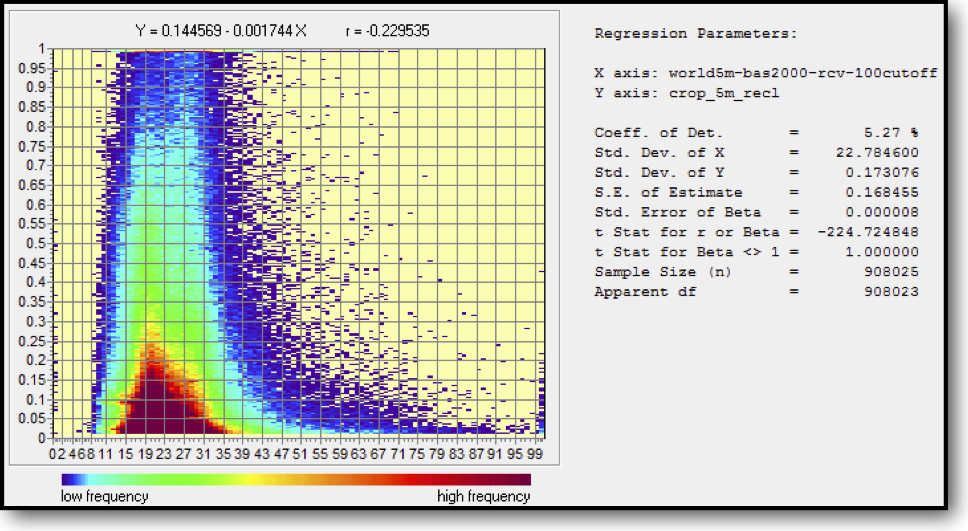
\includegraphics{../assets/cropping_extent_vs_rainfall_cv.png}}

The top panel demonstrates how rainfall CV (on the x-axis) relates to
the probability of crop failure in dryland agricultural systems
(y-axis). The bottom panel provides the distribution of rainfall values
and cropping extent (\% area occupied by crops) across Sub-Saharan
Africa. Rather than depicting a scatterplot, the varying color
represents the density of observations in each portion of the graph's
coordinate space.

Based on the upper panel, we can analyze various stations around
Laikipia to see how they compare to the CV thresholds.

✏️ DIY Code: Use our code from Chapter 2 to analyze the simulated CV of
growing season rainfall for different stations across Laikpia.

💡 Hint: You can use our model analyses to determine optimal planting
dates for any station. Running the model gives a suite of seasonal
rainfall amounts from which you can determin the CV of seasonal rainfall
amounts.

    \begin{Verbatim}[commandchars=\\\{\}]
{\color{incolor}In [{\color{incolor} }]:} \PY{c+c1}{\PYZsh{} This cell intentionally left blank}
\end{Verbatim}


    \hypertarget{coupling-rainfall-variability-water-availability-and-yield}{%
\subsection{Coupling rainfall variability, water availability, and
yield}\label{coupling-rainfall-variability-water-availability-and-yield}}

Our next step will be to develop a relationship between soil water
availability and yield. Most annual crops require a minimuim amount of
soil moisture to avoid wilting. Furthermore, prolonged periods of
wilting/stress are likely to cause complete crop failure.

We can specify a threshold of water resource scarcity, and/or a maximum
duration of water scarcity that would lead to crop failure and use our
same analysis framework to examine how our system responds. We don't
need to change our model, we only need to analyze our results.

Let's say that for any variety, at least \textbf{10 mm} of water is
necessary to avoid wilting. For our soil, 10 mm corresponds to a
volumetric soil moisture of 5\%, which is pretty dry. In addition, let's
say that any season with more the 25\% of the days are below this
threshold leads to crop failure.

Let's define these two new variables as \(S_{wp}=10\), the soil water
amount associated with wilting point) and \(T_{wp}=0.25*T_{harvest}\),
the maximum amount of time at or below wilting point before crops fail.

✏️ DIY Code: Use the \(S_{wp}\) and \(T_{wp}\) values to determine the
likelihood of crop failure based on planting date.

💡 Hint: Since we haven't changed the model - only how we interpret the
data - you can use the same output we've already generated for our
earlier analyses.

    \begin{Verbatim}[commandchars=\\\{\}]
{\color{incolor}In [{\color{incolor} }]:} \PY{c+c1}{\PYZsh{} This cell intentionally left blank.}
\end{Verbatim}



    % Add a bibliography block to the postdoc
    
    
    
    \end{document}
